\documentclass[aspectratio=169,10pt]{beamer}

% Modern professional theme for computer vision presentation
\usetheme{metropolis}
\usecolortheme{default}

% Custom color scheme optimized for computer vision presentation
\definecolor{primaryblue}{RGB}{20,75,140}
\definecolor{secondaryblue}{RGB}{70,130,180}
\definecolor{accentorange}{RGB}{230,95,45}
\definecolor{lightgray}{RGB}{245,245,245}
\definecolor{darkgray}{RGB}{45,45,45}

% Metropolis color customization
\setbeamercolor{progress bar}{fg=primaryblue,bg=lightgray}
\setbeamercolor{title separator}{fg=primaryblue}
\setbeamercolor{progress bar in head/foot}{fg=primaryblue}
\setbeamercolor{progress bar in section page}{fg=primaryblue}
\setbeamercolor{frametitle}{bg=primaryblue,fg=white}
\setbeamercolor{title}{fg=primaryblue}
\setbeamercolor{subtitle}{fg=secondaryblue}
\setbeamercolor{structure}{fg=primaryblue}
\setbeamercolor{alerted text}{fg=accentorange}
\setbeamercolor{block title}{bg=primaryblue,fg=white}
\setbeamercolor{block body}{bg=lightgray,fg=darkgray}
\setbeamercolor{block title alerted}{bg=accentorange,fg=white}
\setbeamercolor{block body alerted}{bg=lightgray,fg=darkgray}

% Enhanced packages for mathematical rigor
\usepackage{amsmath,amssymb,amsfonts}
\usepackage{graphicx}
\usepackage{booktabs}
\usepackage{xcolor}
\usepackage{tikz}
\usepackage{algorithm2e}

% Professional formatting
\setbeamertemplate{navigation symbols}{}
\setbeamertemplate{footline}[frame number]

% Title information
\title{Basic Enhancement in Digital Image Processing}
\subtitle{CMSC 178IP - Comprehensive Study Guide}
\author{Digital Image Processing Course}
\institute{Computer Science Department}
\date{\today}

\begin{document}

% Title slide
\begin{frame}
\titlepage
\end{frame}

% Table of contents
\begin{frame}{Course Outline}
\tableofcontents
\end{frame}

\section{Introduction}

\begin{frame}{What is Image Enhancement?}
\begin{alertblock}{Definition}
Image enhancement aims to improve the visual appearance of images or convert images to a form better suited for analysis by humans or machines.
\end{alertblock}

\textbf{Mathematical Foundation:}
$$g(x,y) = T[f(x,y)]$$

Where:
\begin{itemize}
\item $f(x,y)$ = input image
\item $g(x,y)$ = output (enhanced) image
\item $T$ = transformation operator
\end{itemize}

\textbf{Enhancement Categories:}
\begin{itemize}
\item Spatial domain techniques
\item Frequency domain techniques
\item Point operations
\item Neighborhood operations
\end{itemize}
\end{frame}

\begin{frame}{Problem Setup and Motivation}
\textbf{Why do we need image enhancement?}

\begin{columns}
\column{0.6\textwidth}
\begin{itemize}
\item Poor lighting conditions
\item Sensor limitations
\item Noise interference
\item Low contrast
\item Blurring effects
\item Color distortions
\end{itemize}

\textbf{Applications:}
\begin{itemize}
\item Medical imaging
\item Satellite imagery
\item Photography
\item Security systems
\item Machine vision
\end{itemize}

\column{0.4\textwidth}
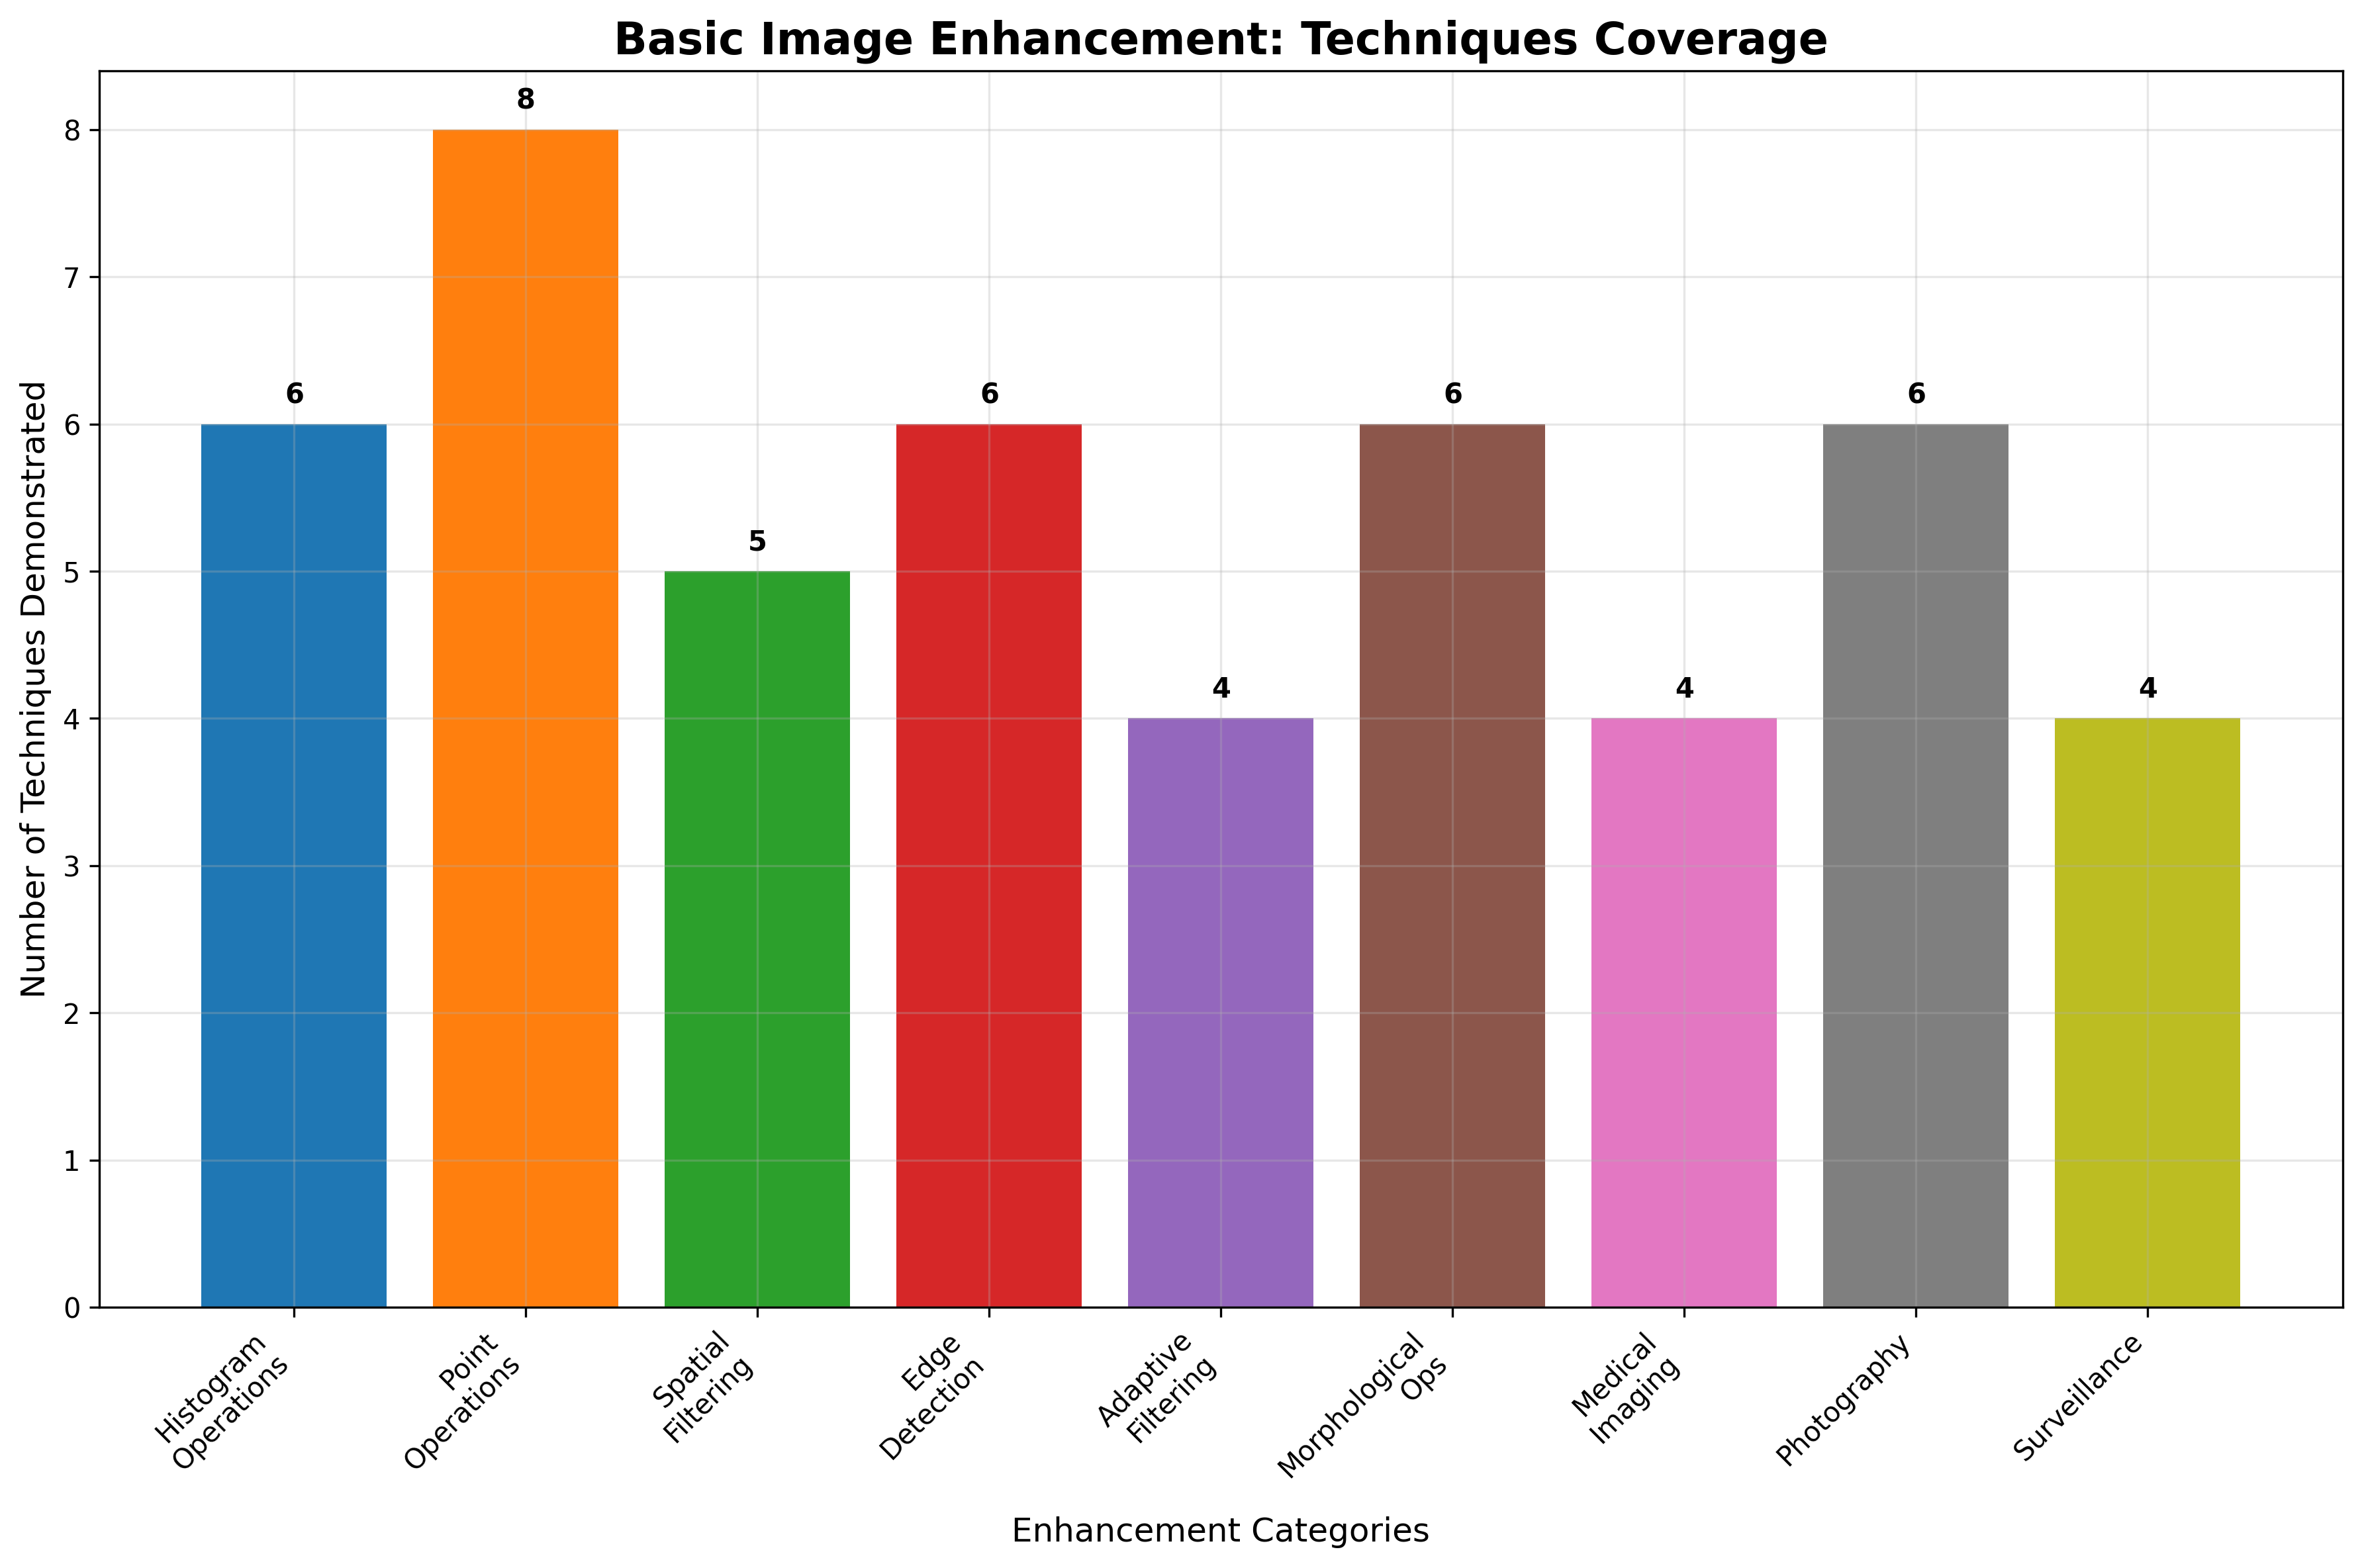
\includegraphics[width=\textwidth]{../figures/enhancement_summary.png}\\
\centering{\small Enhancement techniques coverage across different categories}
\end{columns}
\end{frame}

\section{Core Theory}

\begin{frame}{Histogram Analysis}
\begin{columns}
\begin{column}{0.5\textwidth}
\begin{alertblock}{Histogram Definition}
A histogram represents the frequency distribution of pixel intensities in an image.
\end{alertblock}

\textbf{Mathematical Formulation:}
$$h(r_k) = n_k$$

Where:
\begin{itemize}
\item $r_k$ = $k$-th intensity level
\item $n_k$ = number of pixels with intensity $r_k$
\end{itemize}

\textbf{Normalized Histogram:}
$$p(r_k) = \frac{n_k}{MN} = \frac{h(r_k)}{MN}$$

Where $M \times N$ is the total number of pixels.
\end{column}
\begin{column}{0.45\textwidth}
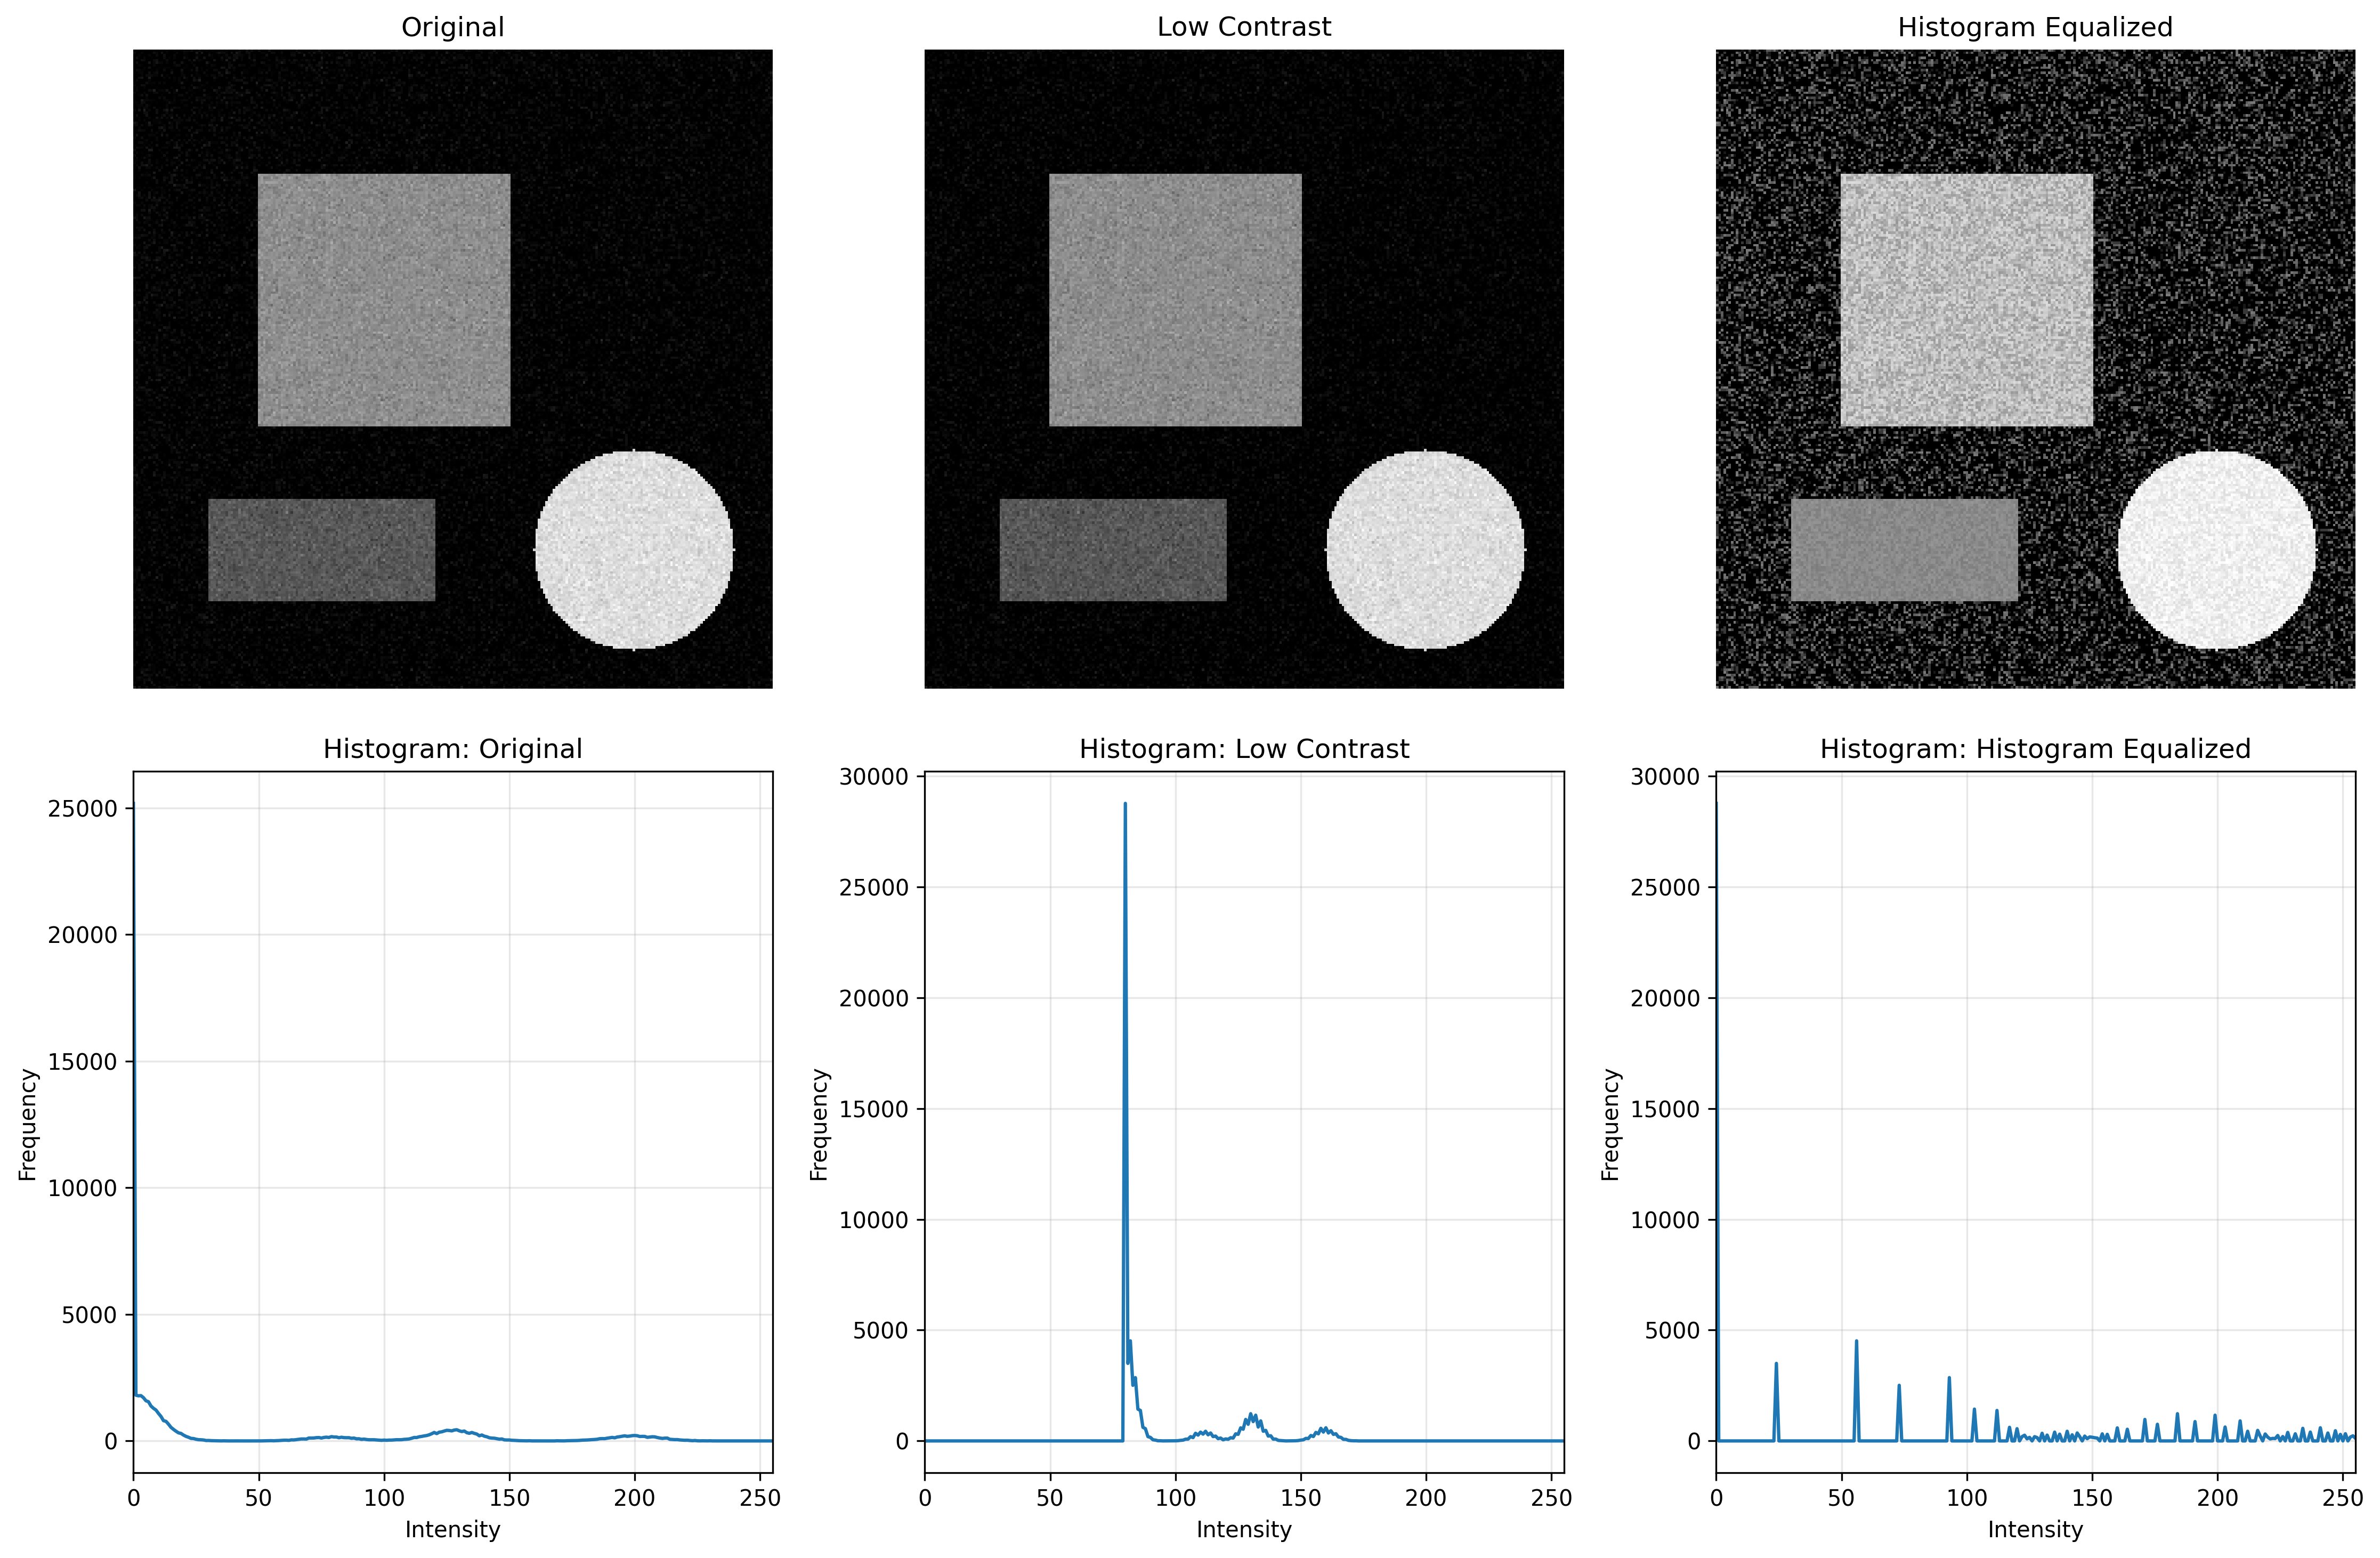
\includegraphics[width=\textwidth]{../figures/histogram_operations.png}\\
\centering{\small Original vs. enhanced histograms showing distribution changes}
\end{column}
\end{columns}
\end{frame}

\begin{frame}{Histogram Equalization}
\begin{columns}
\begin{column}{0.55\textwidth}
\textbf{Goal:} Redistribute pixel intensities to achieve uniform histogram

\textbf{Transformation Function:}
$$s = T(r) = (L-1) \sum_{j=0}^{r} p_r(j)$$

Where:
\begin{itemize}
\item $L$ = number of intensity levels
\item $s$ = output intensity
\item $r$ = input intensity
\end{itemize}
\end{column}
\begin{column}{0.4\textwidth}
\begin{alertblock}{Algorithm Steps}
\begin{enumerate}
\item Compute histogram $h(r_k)$
\item Calculate CDF
\item Normalize to $[0, L-1]$
\item Apply lookup table
\end{enumerate}
\end{alertblock}
\end{column}
\end{columns}
\end{frame}

\begin{frame}{Point Operations Theory}
\begin{columns}
\begin{column}{0.55\textwidth}
\textbf{General Form:} $s = T(r)$

\textbf{Common Transformations:}

\begin{align}
\text{Linear:} \quad s &= ar + b \\
\text{Power Law (Gamma):} \quad s &= cr^\gamma \\
\text{Logarithmic:} \quad s &= c \log(1 + r) \\
\text{Exponential:} \quad s &= c(b^r - 1)
\end{align}

\begin{alertblock}{Gamma Correction}
Controls image brightness and contrast simultaneously:
\begin{itemize}
\item $\gamma < 1$: brightens image
\item $\gamma > 1$: darkens image
\item $\gamma = 1$: no change (linear)
\end{itemize}
\end{alertblock}
\end{column}
\begin{column}{0.4\textwidth}
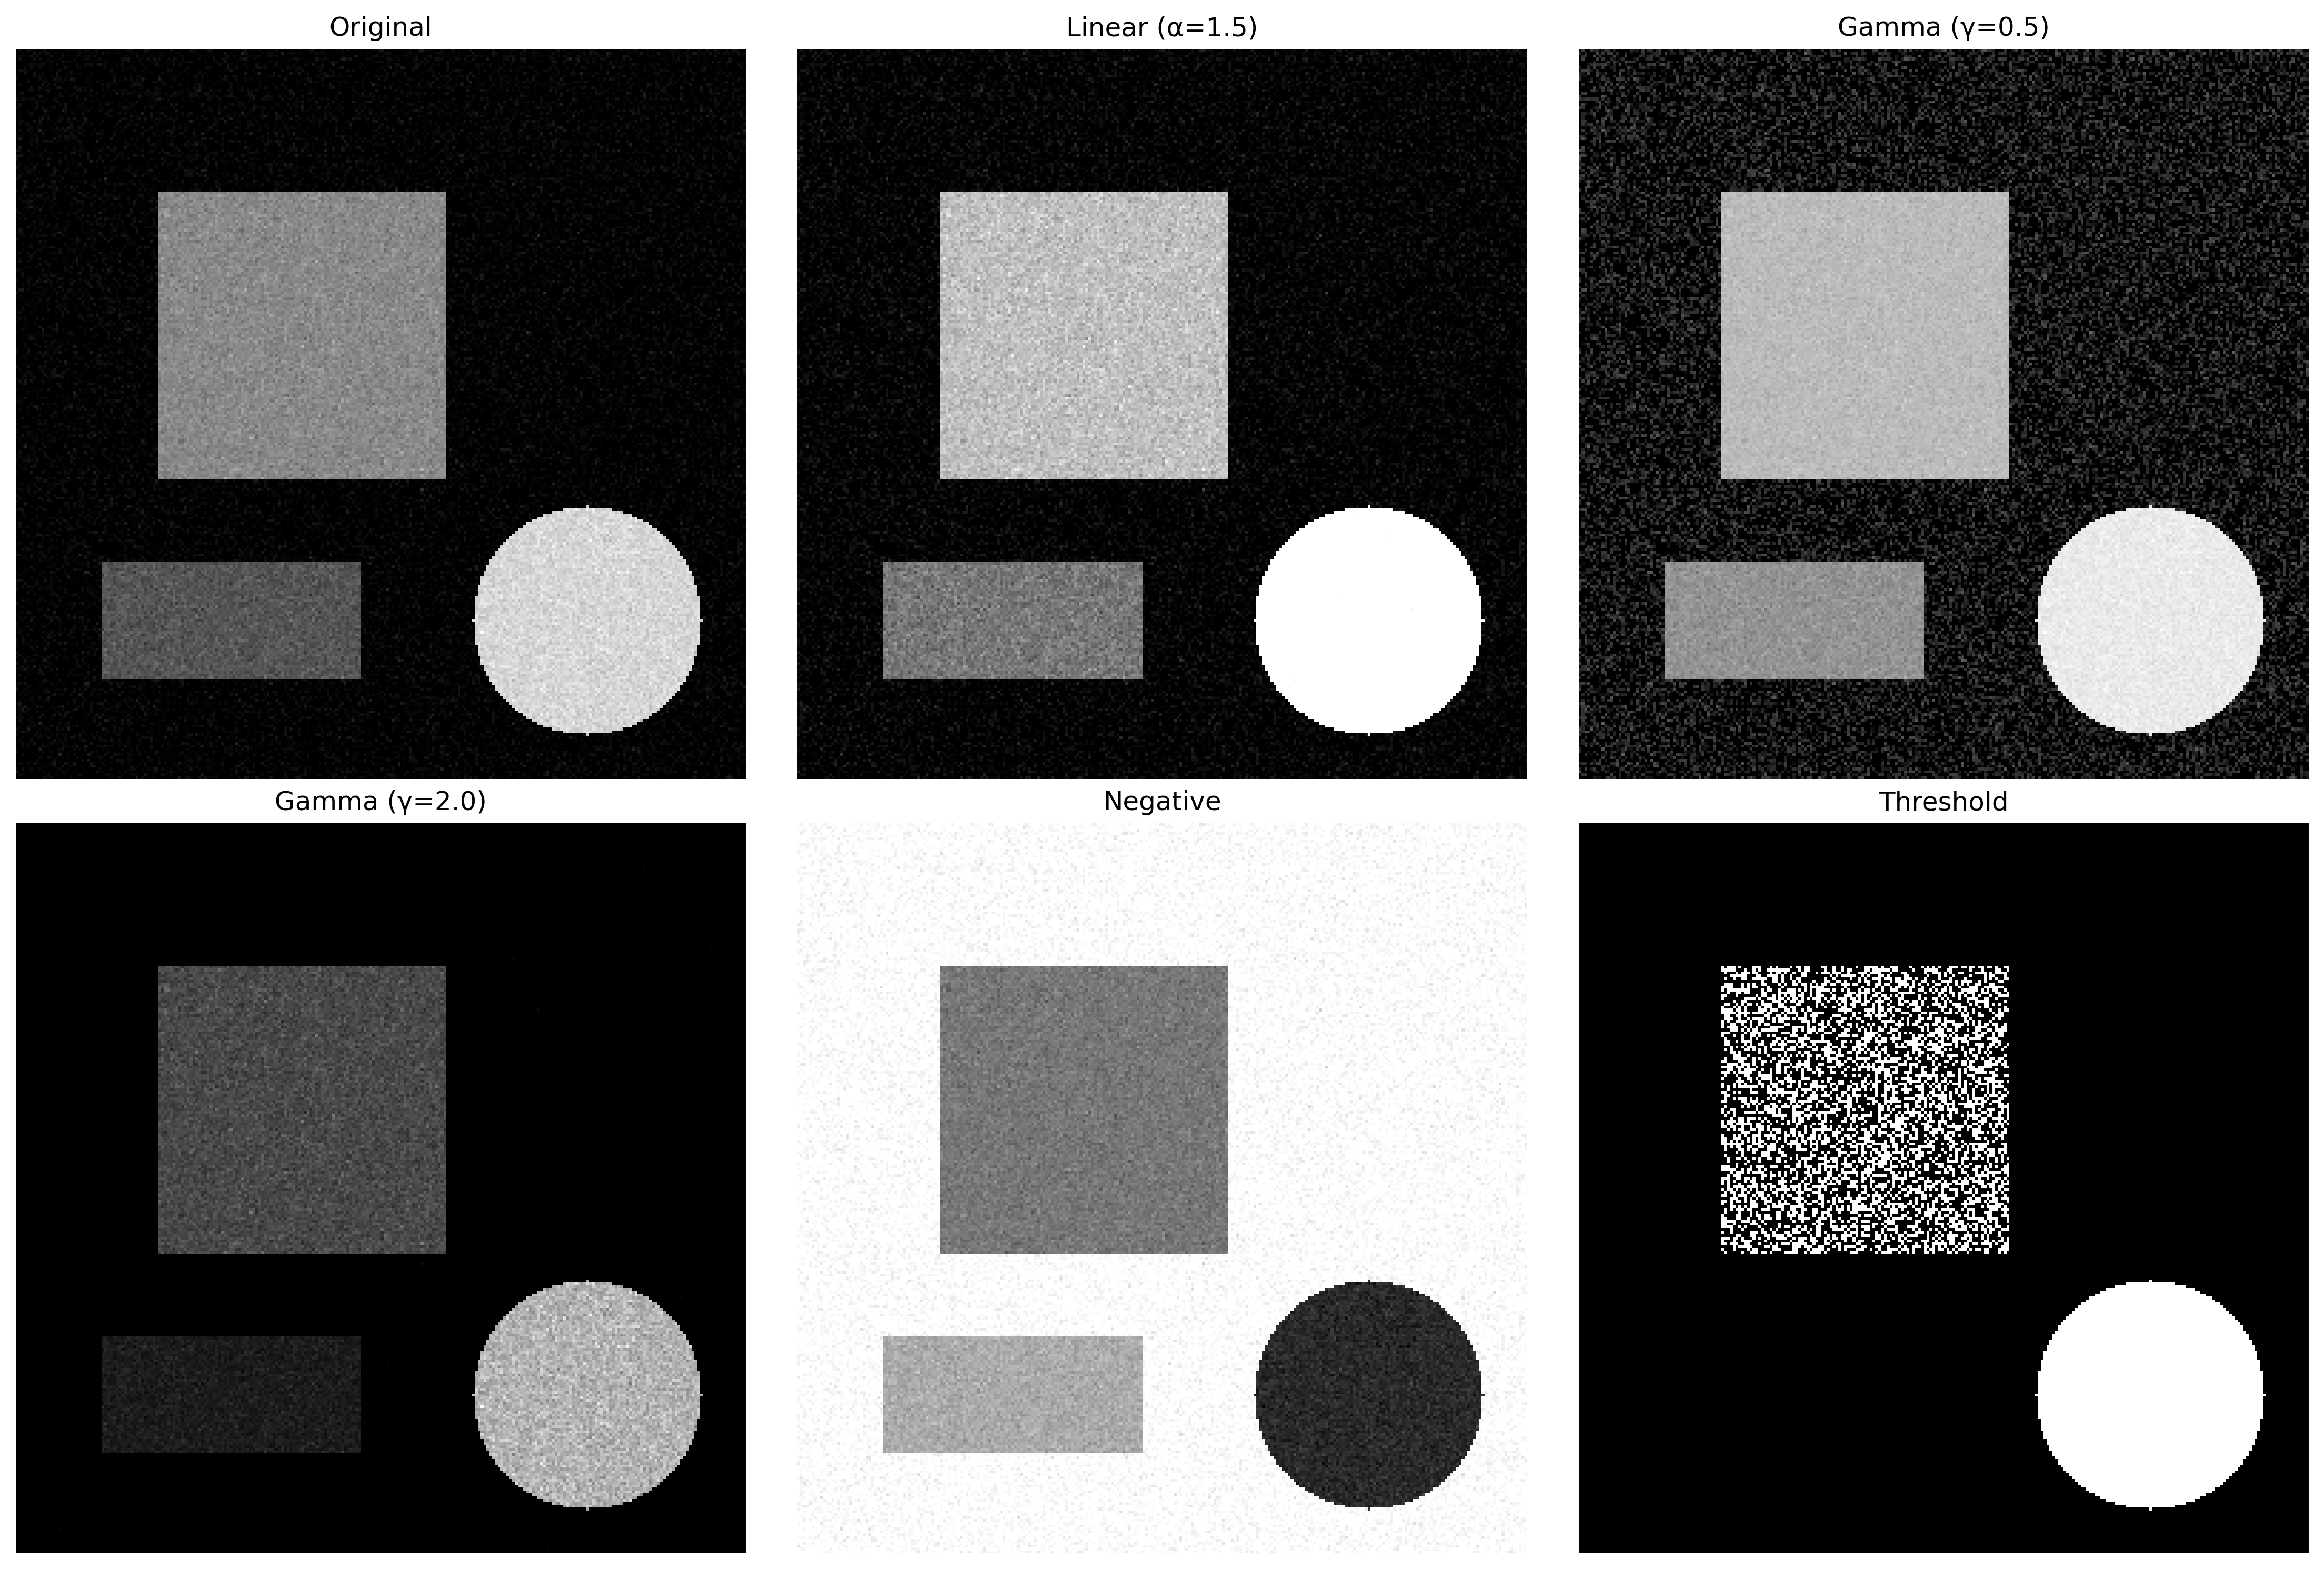
\includegraphics[width=\textwidth]{../figures/point_operations.png}\\
\centering{\small Point operation effects: linear, gamma, and logarithmic transformations}
\end{column}
\end{columns}
\end{frame}

\section{Methods and Algorithms}

\begin{frame}{Spatial Filtering Fundamentals}
\begin{columns}
\begin{column}{0.5\textwidth}
\textbf{Convolution Operation:}
$$g(x,y) = w \star f = \sum_{s=-a}^{a} \sum_{t=-b}^{b} w(s,t) f(x+s, y+t)$$

Where:
\begin{itemize}
\item $w$ = filter mask/kernel
\item $f$ = input image
\item $(2a+1) \times (2b+1)$ = mask size
\end{itemize}

\textbf{Filter Categories:}
\begin{itemize}
\item \textbf{Smoothing:} Remove noise, reduce detail
\item \textbf{Sharpening:} Enhance edges, increase detail
\item \textbf{Edge Detection:} Highlight discontinuities
\end{itemize}
\end{column}
\begin{column}{0.45\textwidth}
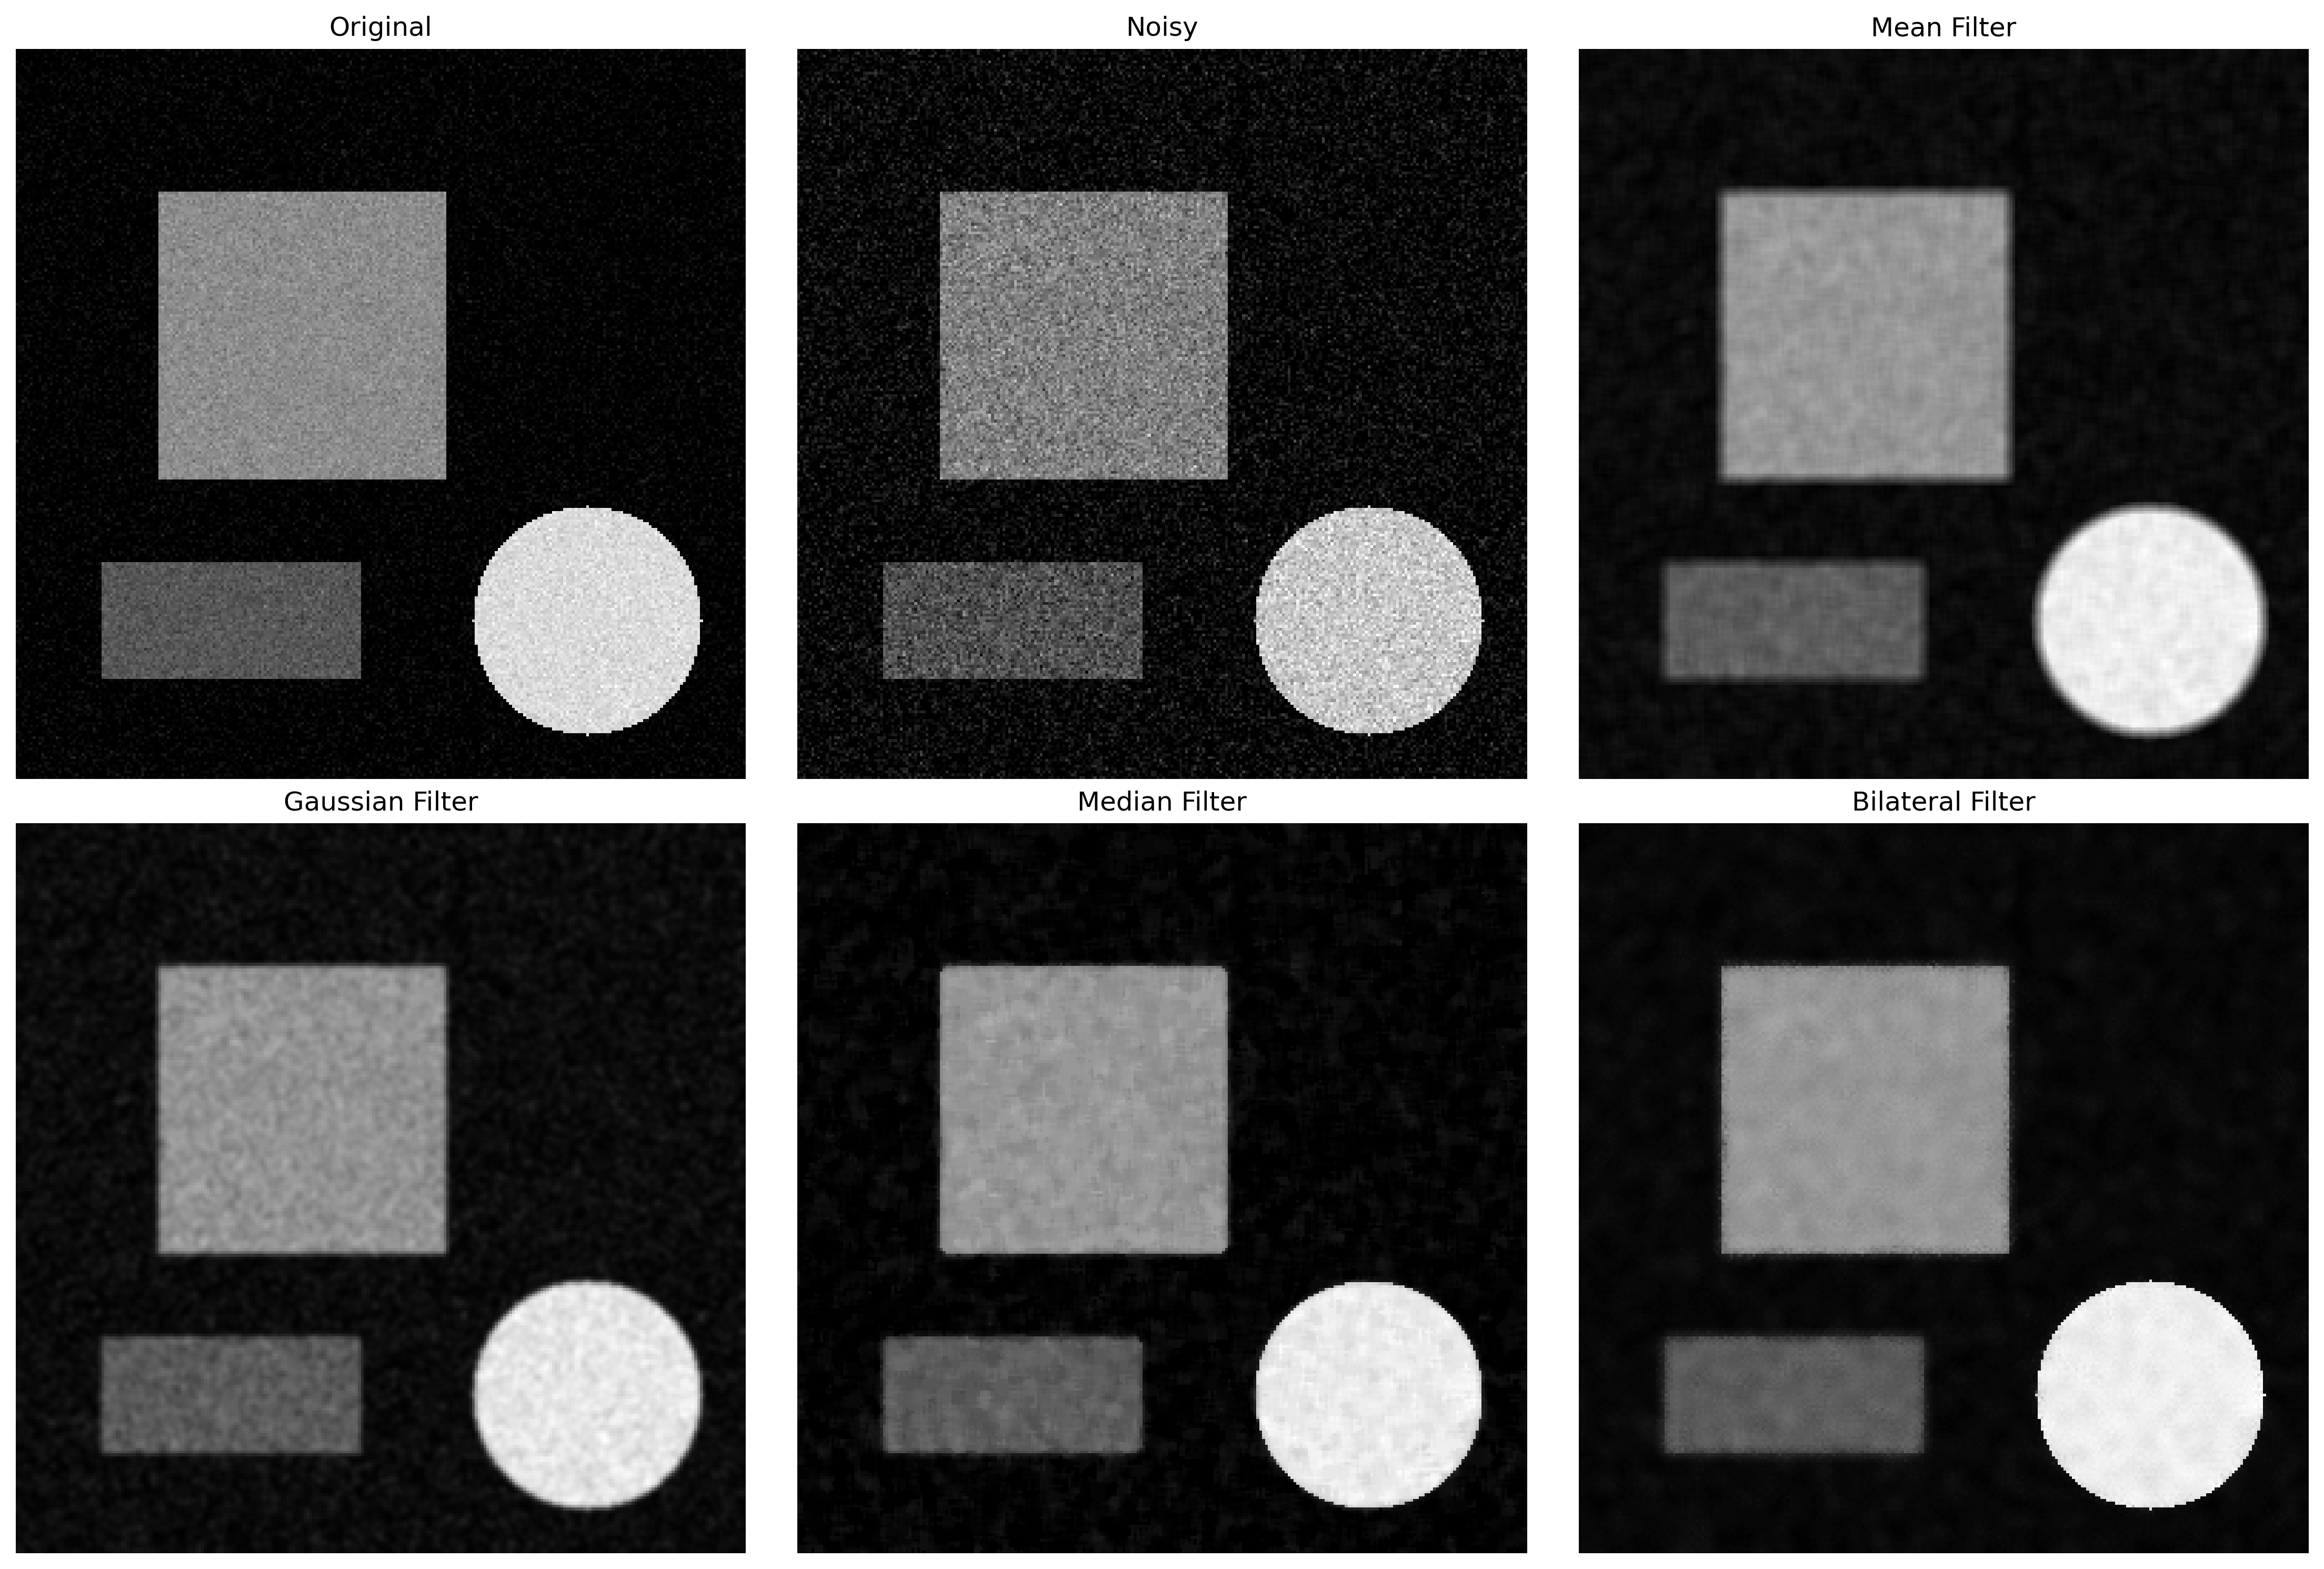
\includegraphics[width=\textwidth]{../figures/spatial_filtering.png}\\
\centering{\small Spatial filtering kernels and their effects on image enhancement}
\end{column}
\end{columns}
\end{frame}

\begin{frame}{Noise Reduction Algorithms}
\begin{columns}
\begin{column}{0.5\textwidth}
\textbf{Linear Filters:}
\begin{align}
\text{Mean:} \quad \hat{f} &= \frac{1}{mn} \sum g(s,t) \\
\text{Gaussian:} \quad G &= \frac{1}{2\pi\sigma^2} e^{-\frac{r^2}{2\sigma^2}}
\end{align}

\textbf{Non-linear Filters:}
\begin{itemize}
\item \textbf{Median:} Neighborhood median
\item \textbf{Bilateral:} Edge-preserving
\item \textbf{Non-local:} Self-similarity
\end{itemize}
\end{column}
\begin{column}{0.45\textwidth}
\begin{alertblock}{Filter Selection}
\begin{itemize}
\item Gaussian noise → Gaussian filter
\item Salt \& pepper → Median filter
\item Edge preservation → Bilateral filter
\end{itemize}
\end{alertblock}
\end{column}
\end{columns}
\end{frame}

\begin{frame}{Edge Detection Operators}
\begin{columns}
\begin{column}{0.55\textwidth}
\textbf{Gradient-based Methods:}

\textbf{Sobel Operator:}
$$G_x = \begin{bmatrix} -1 & 0 & 1 \\ -2 & 0 & 2 \\ -1 & 0 & 1 \end{bmatrix}$$
$$G_y = \begin{bmatrix} -1 & -2 & -1 \\ 0 & 0 & 0 \\ 1 & 2 & 1 \end{bmatrix}$$

\textbf{Gradient Magnitude:}
$$|\nabla f| = \sqrt{G_x^2 + G_y^2}$$

\textbf{Laplacian Operator:}
$$\nabla^2 f = \frac{\partial^2 f}{\partial x^2} + \frac{\partial^2 f}{\partial y^2}$$

\textbf{Discrete Laplacian:}
$$\nabla^2 f = \begin{bmatrix} 0 & 1 & 0 \\ 1 & -4 & 1 \\ 0 & 1 & 0 \end{bmatrix}$$
\end{column}
\begin{column}{0.4\textwidth}
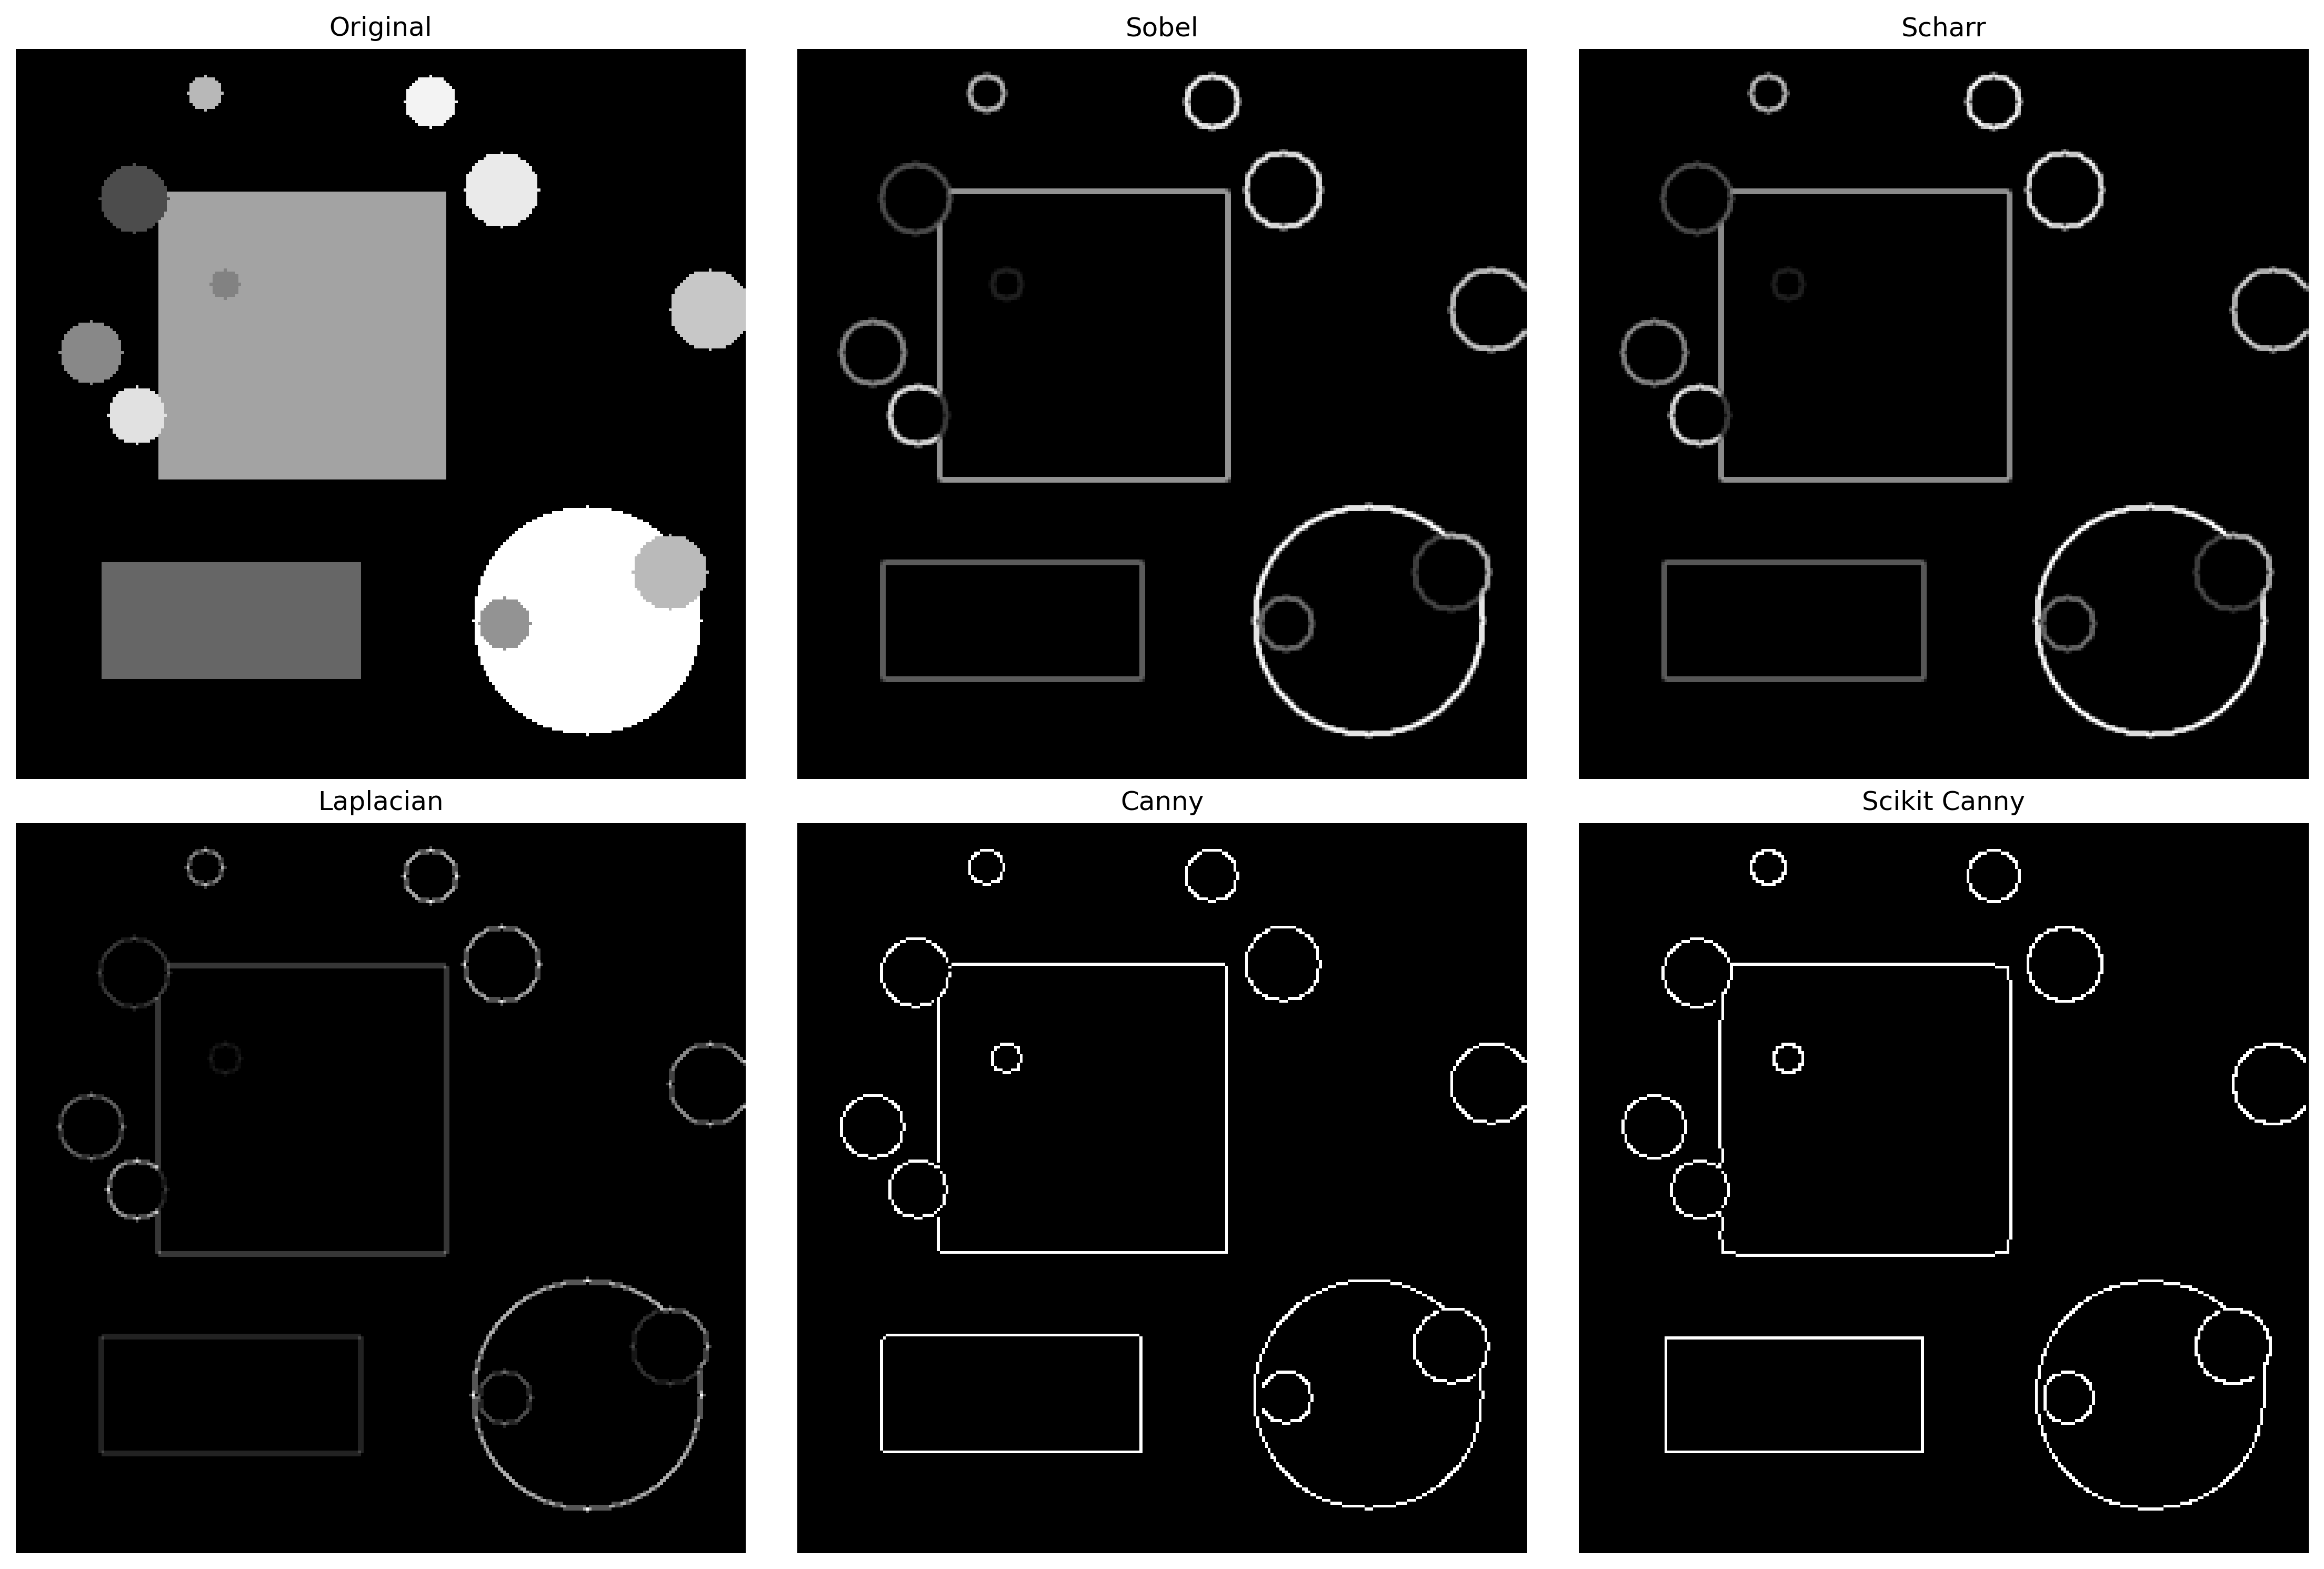
\includegraphics[width=\textwidth]{../figures/edge_detection_advanced.png}\\
\centering{\small Edge detection results: Sobel, Canny, and Laplacian operators}
\end{column}
\end{columns}
\end{frame}

\begin{frame}{Canny Edge Detection Algorithm}
\begin{alertblock}{Multi-Stage Optimal Edge Detector}
\textbf{Criteria:} Good detection, good localization, single response
\end{alertblock}

\textbf{Algorithm Steps:}
\begin{enumerate}
\item \textbf{Smoothing:} Apply Gaussian filter to reduce noise
\item \textbf{Gradient:} Compute gradient magnitude and direction
\item \textbf{Non-maximum suppression:} Thin edges to single pixel width
\item \textbf{Double thresholding:} Use two thresholds (high, low)
\item \textbf{Edge tracking:} Connect edge segments using hysteresis
\end{enumerate}
\end{frame}

\begin{frame}{Canny Algorithm - Mathematical Foundation}
\textbf{Optimal Filter Criteria:}
$$\text{Optimal filter} = \arg\max \left( \frac{S}{N} \cdot L \cdot \frac{1}{W} \right)$$

Where:
\begin{itemize}
\item $S/N$ = Signal-to-noise ratio
\item $L$ = Localization factor
\item $W$ = Multiple response factor
\end{itemize}

\textbf{Key Properties:}
\begin{itemize}
\item \textbf{Good detection:} Minimize false positives and negatives
\item \textbf{Good localization:} Detected edges close to true edges
\item \textbf{Single response:} One response per edge
\end{itemize}
\end{frame}

\section{Applications}

\begin{frame}{Medical Imaging Enhancement}
\begin{columns}
\begin{column}{0.45\textwidth}
\textbf{Challenges in Medical Imaging:}
\begin{itemize}
\item Low contrast between tissues
\item Noise from acquisition systems
\item Need for subtle detail enhancement
\item Preservation of diagnostic information
\end{itemize}

\textbf{Common Techniques:}
\begin{itemize}
\item \textbf{CLAHE:} Contrast Limited Adaptive Histogram Equalization
\item \textbf{Gamma correction:} Adjust brightness/contrast
\item \textbf{Noise reduction:} Bilateral, non-local means
\item \textbf{Edge enhancement:} Unsharp masking
\end{itemize}
\end{column}
\begin{column}{0.5\textwidth}
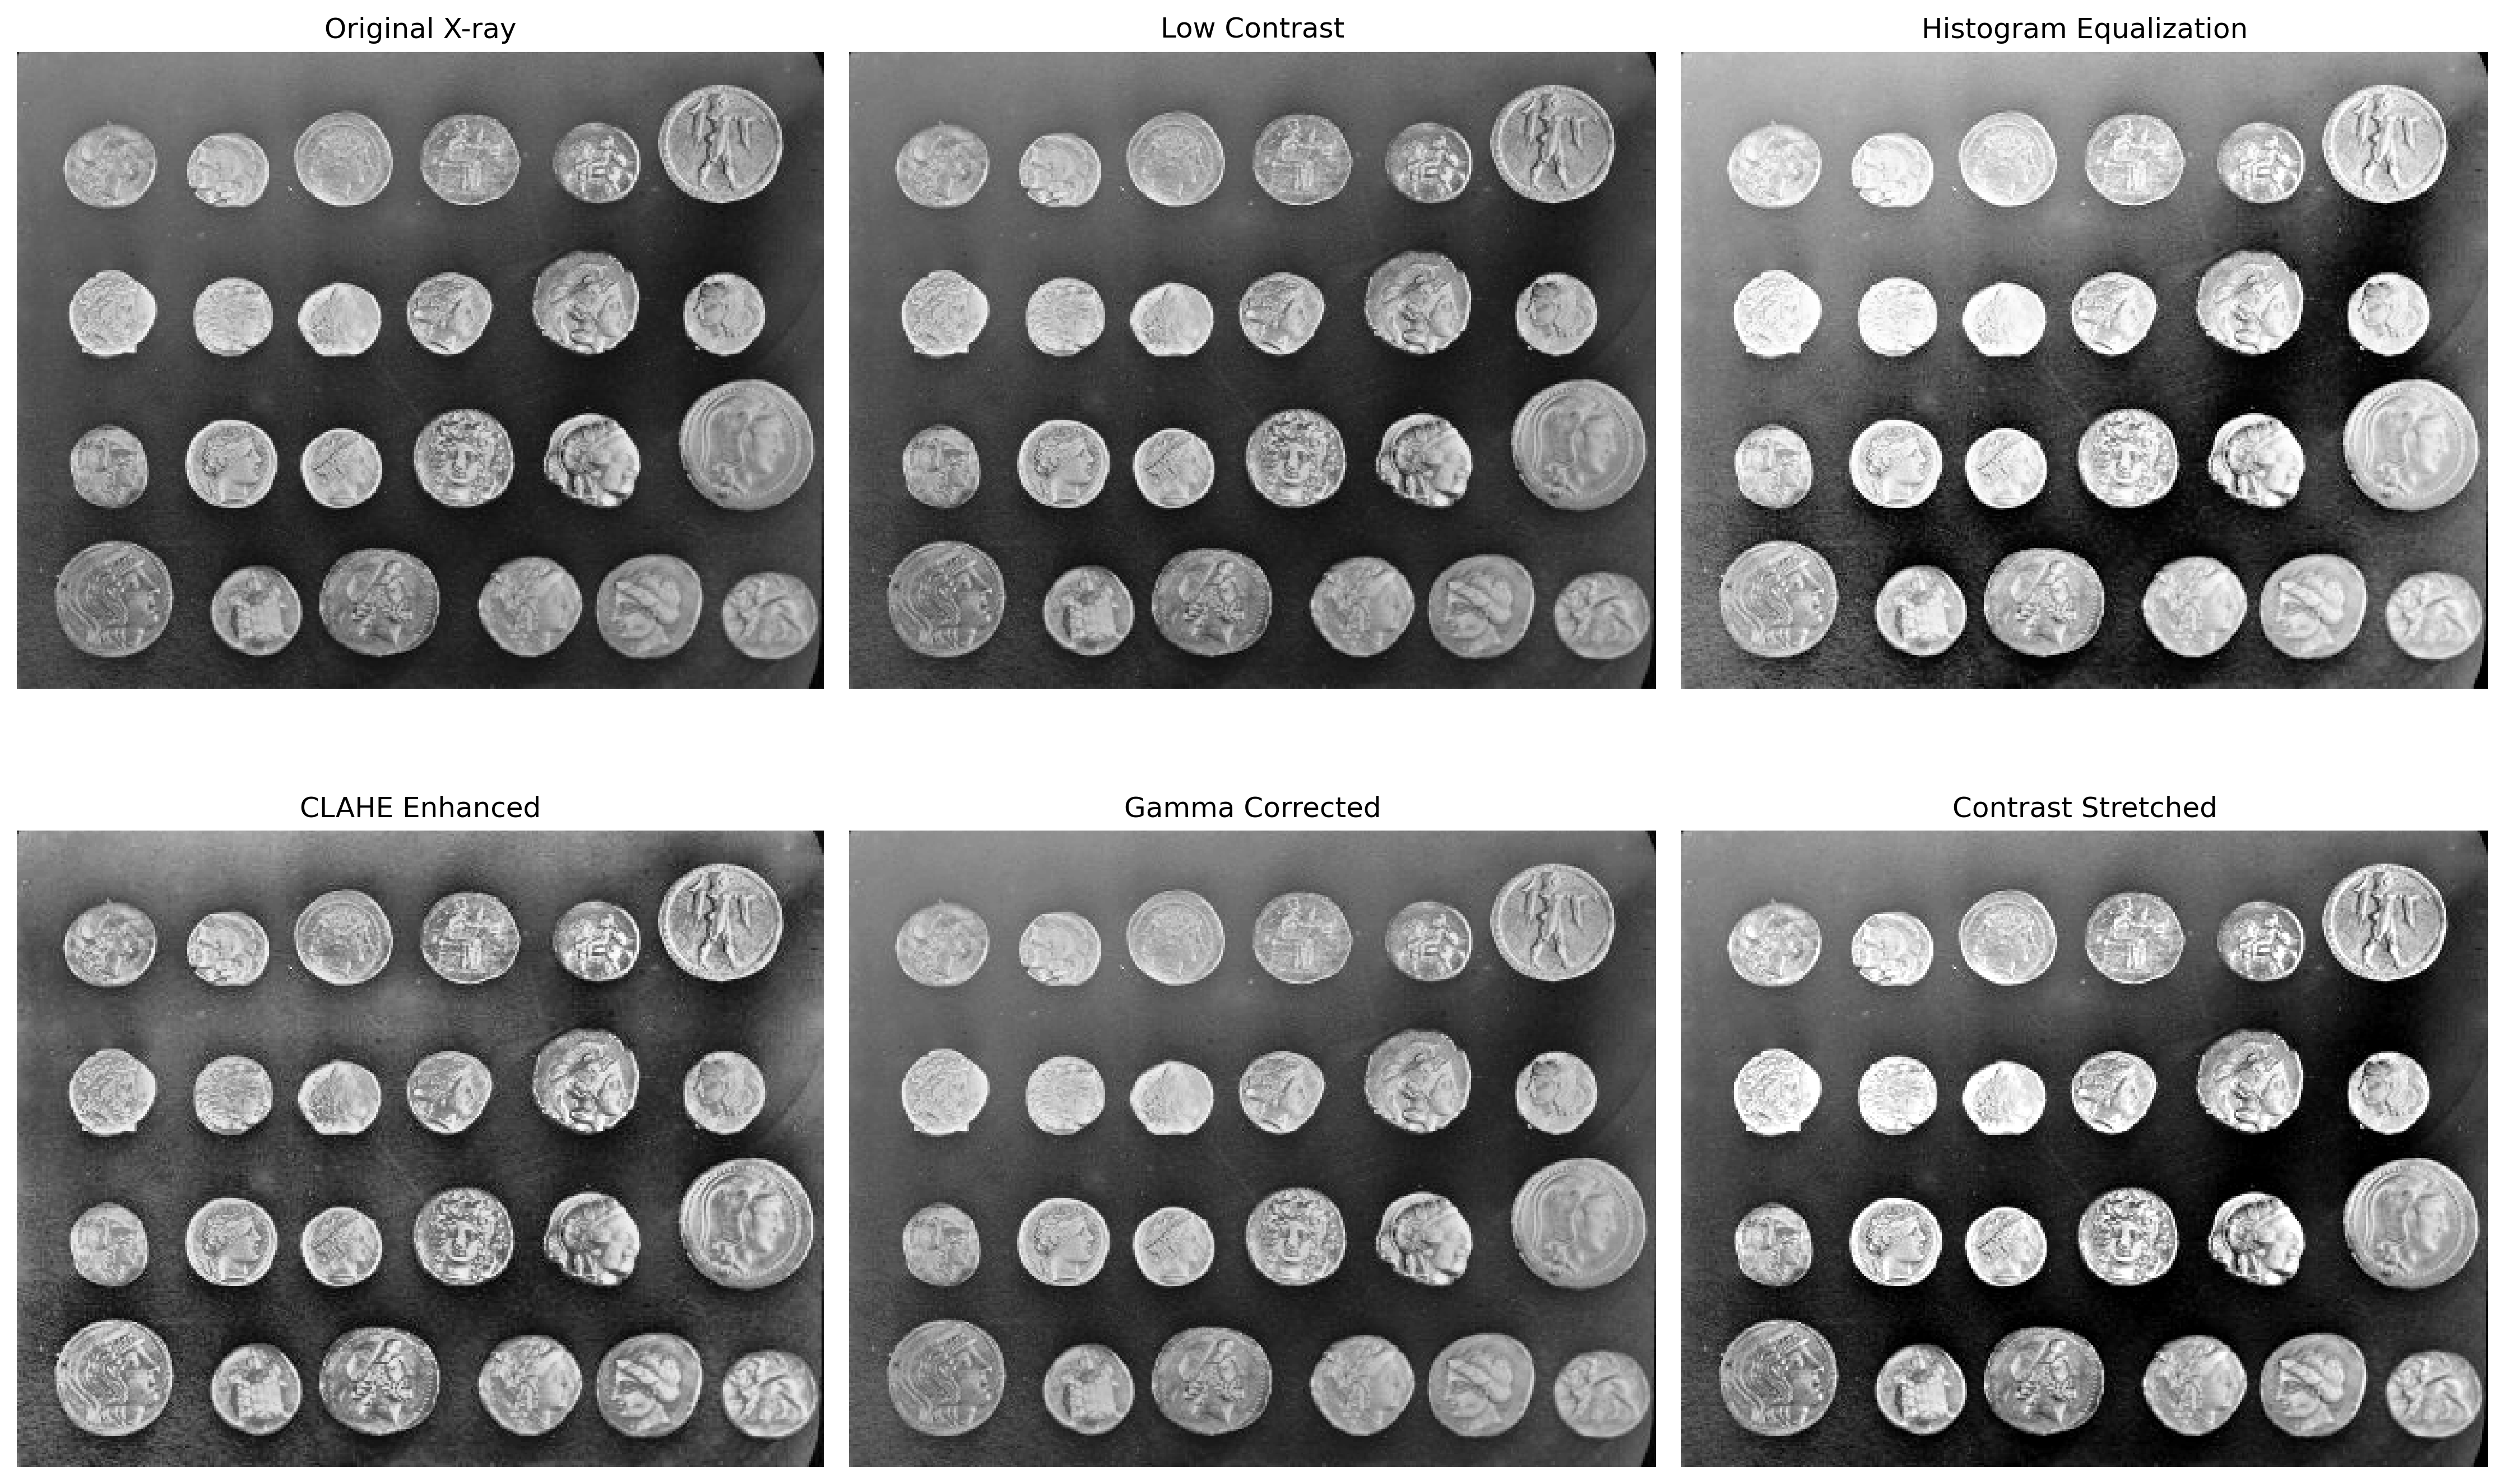
\includegraphics[width=\textwidth]{../figures/medical_imaging_enhancement.png}\\
\centering{\small Medical image enhancement: original, CLAHE, and gamma corrected}
\end{column}
\end{columns}
\end{frame}

\begin{frame}{Photography and Consumer Applications}
\begin{columns}
\begin{column}{0.45\textwidth}
\textbf{Enhancement Goals:}
\begin{itemize}
\item Improve visual appeal
\item Correct exposure issues
\item Enhance colors and contrast
\item Reduce noise
\end{itemize}

\textbf{Techniques:}
\begin{itemize}
\item \textbf{Histogram equalization:} Improve contrast
\item \textbf{Gamma correction:} Adjust brightness
\item \textbf{Saturation enhancement:} Boost colors
\item \textbf{Sharpening:} Increase perceived detail
\end{itemize}
\end{column}
\begin{column}{0.5\textwidth}
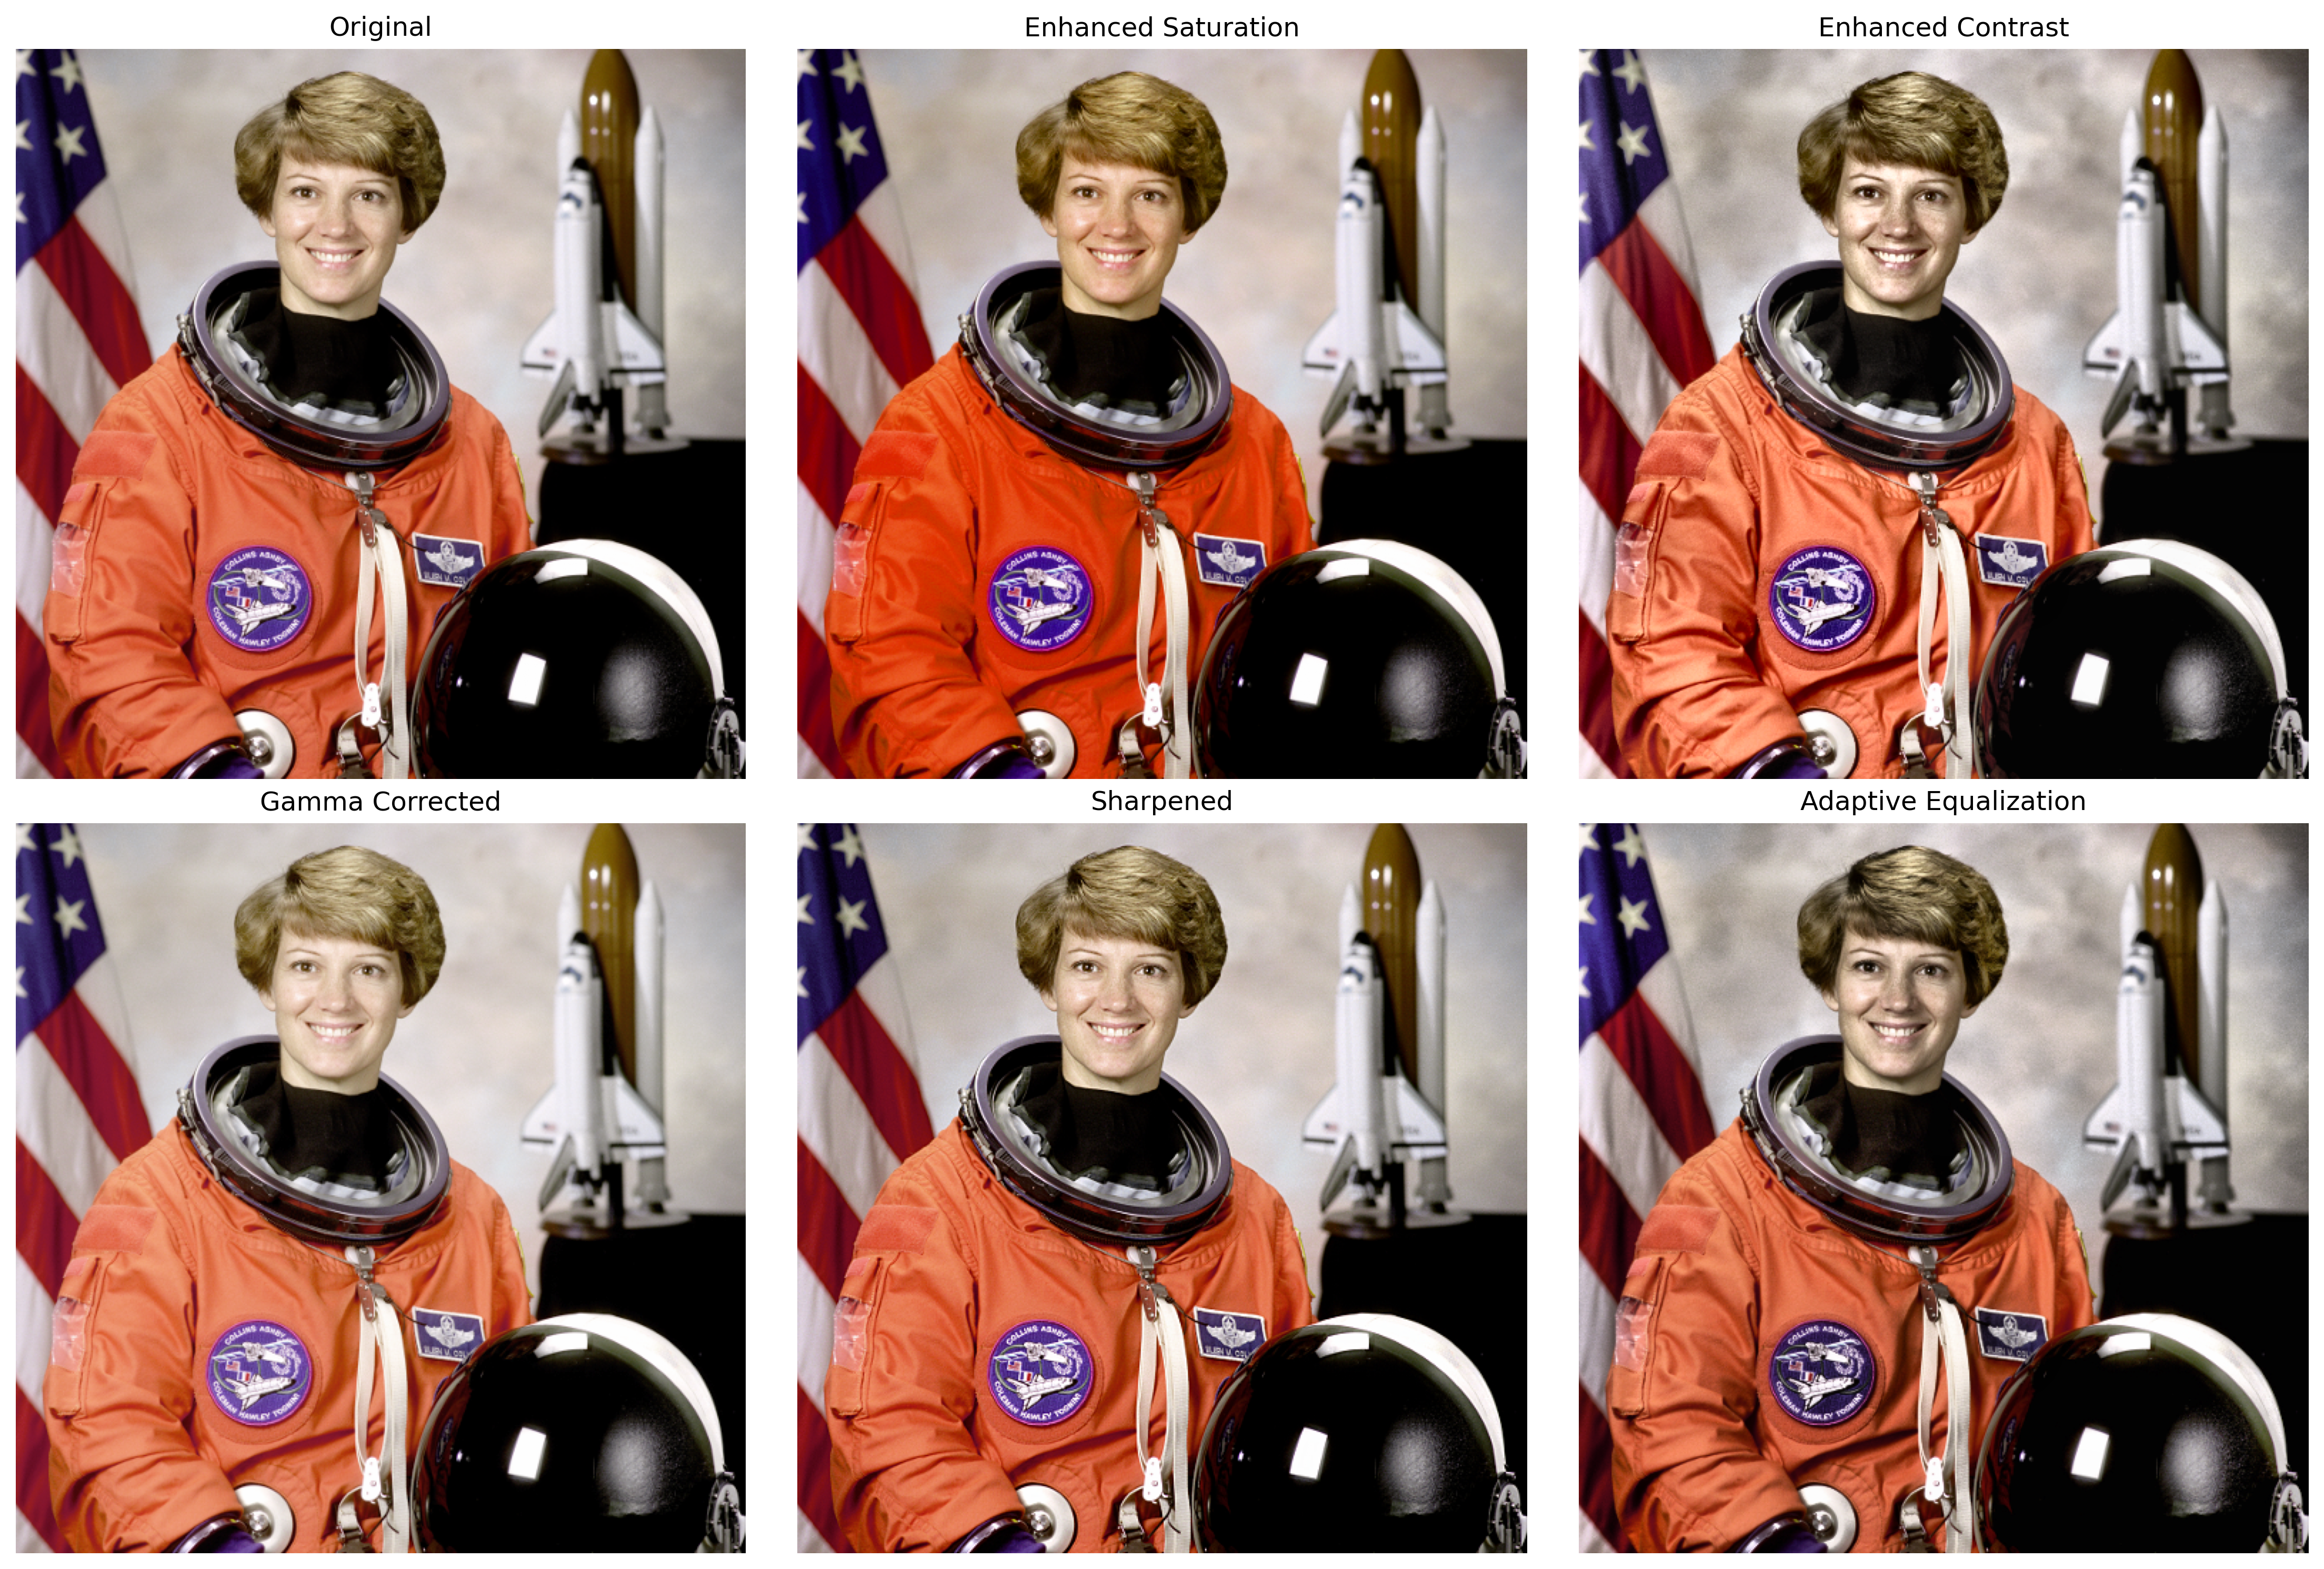
\includegraphics[width=\textwidth]{../figures/photography_enhancement.png}\\
\centering{\small Photography enhancement: contrast adjustment, color correction, and sharpening}
\end{column}
\end{columns}
\end{frame}

\begin{frame}{Surveillance and Security}
\begin{columns}
\begin{column}{0.45\textwidth}
\textbf{Challenges:}
\begin{itemize}
\item Poor lighting conditions
\item High noise levels
\item Need for feature recognition
\item Real-time processing requirements
\end{itemize}

\textbf{Enhancement Pipeline:}
\begin{enumerate}
\item \textbf{Noise reduction:} Bilateral filtering
\item \textbf{Contrast enhancement:} CLAHE
\item \textbf{Edge enhancement:} For feature detection
\item \textbf{Histogram stretching:} Improve dynamic range
\end{enumerate}
\end{column}
\begin{column}{0.5\textwidth}
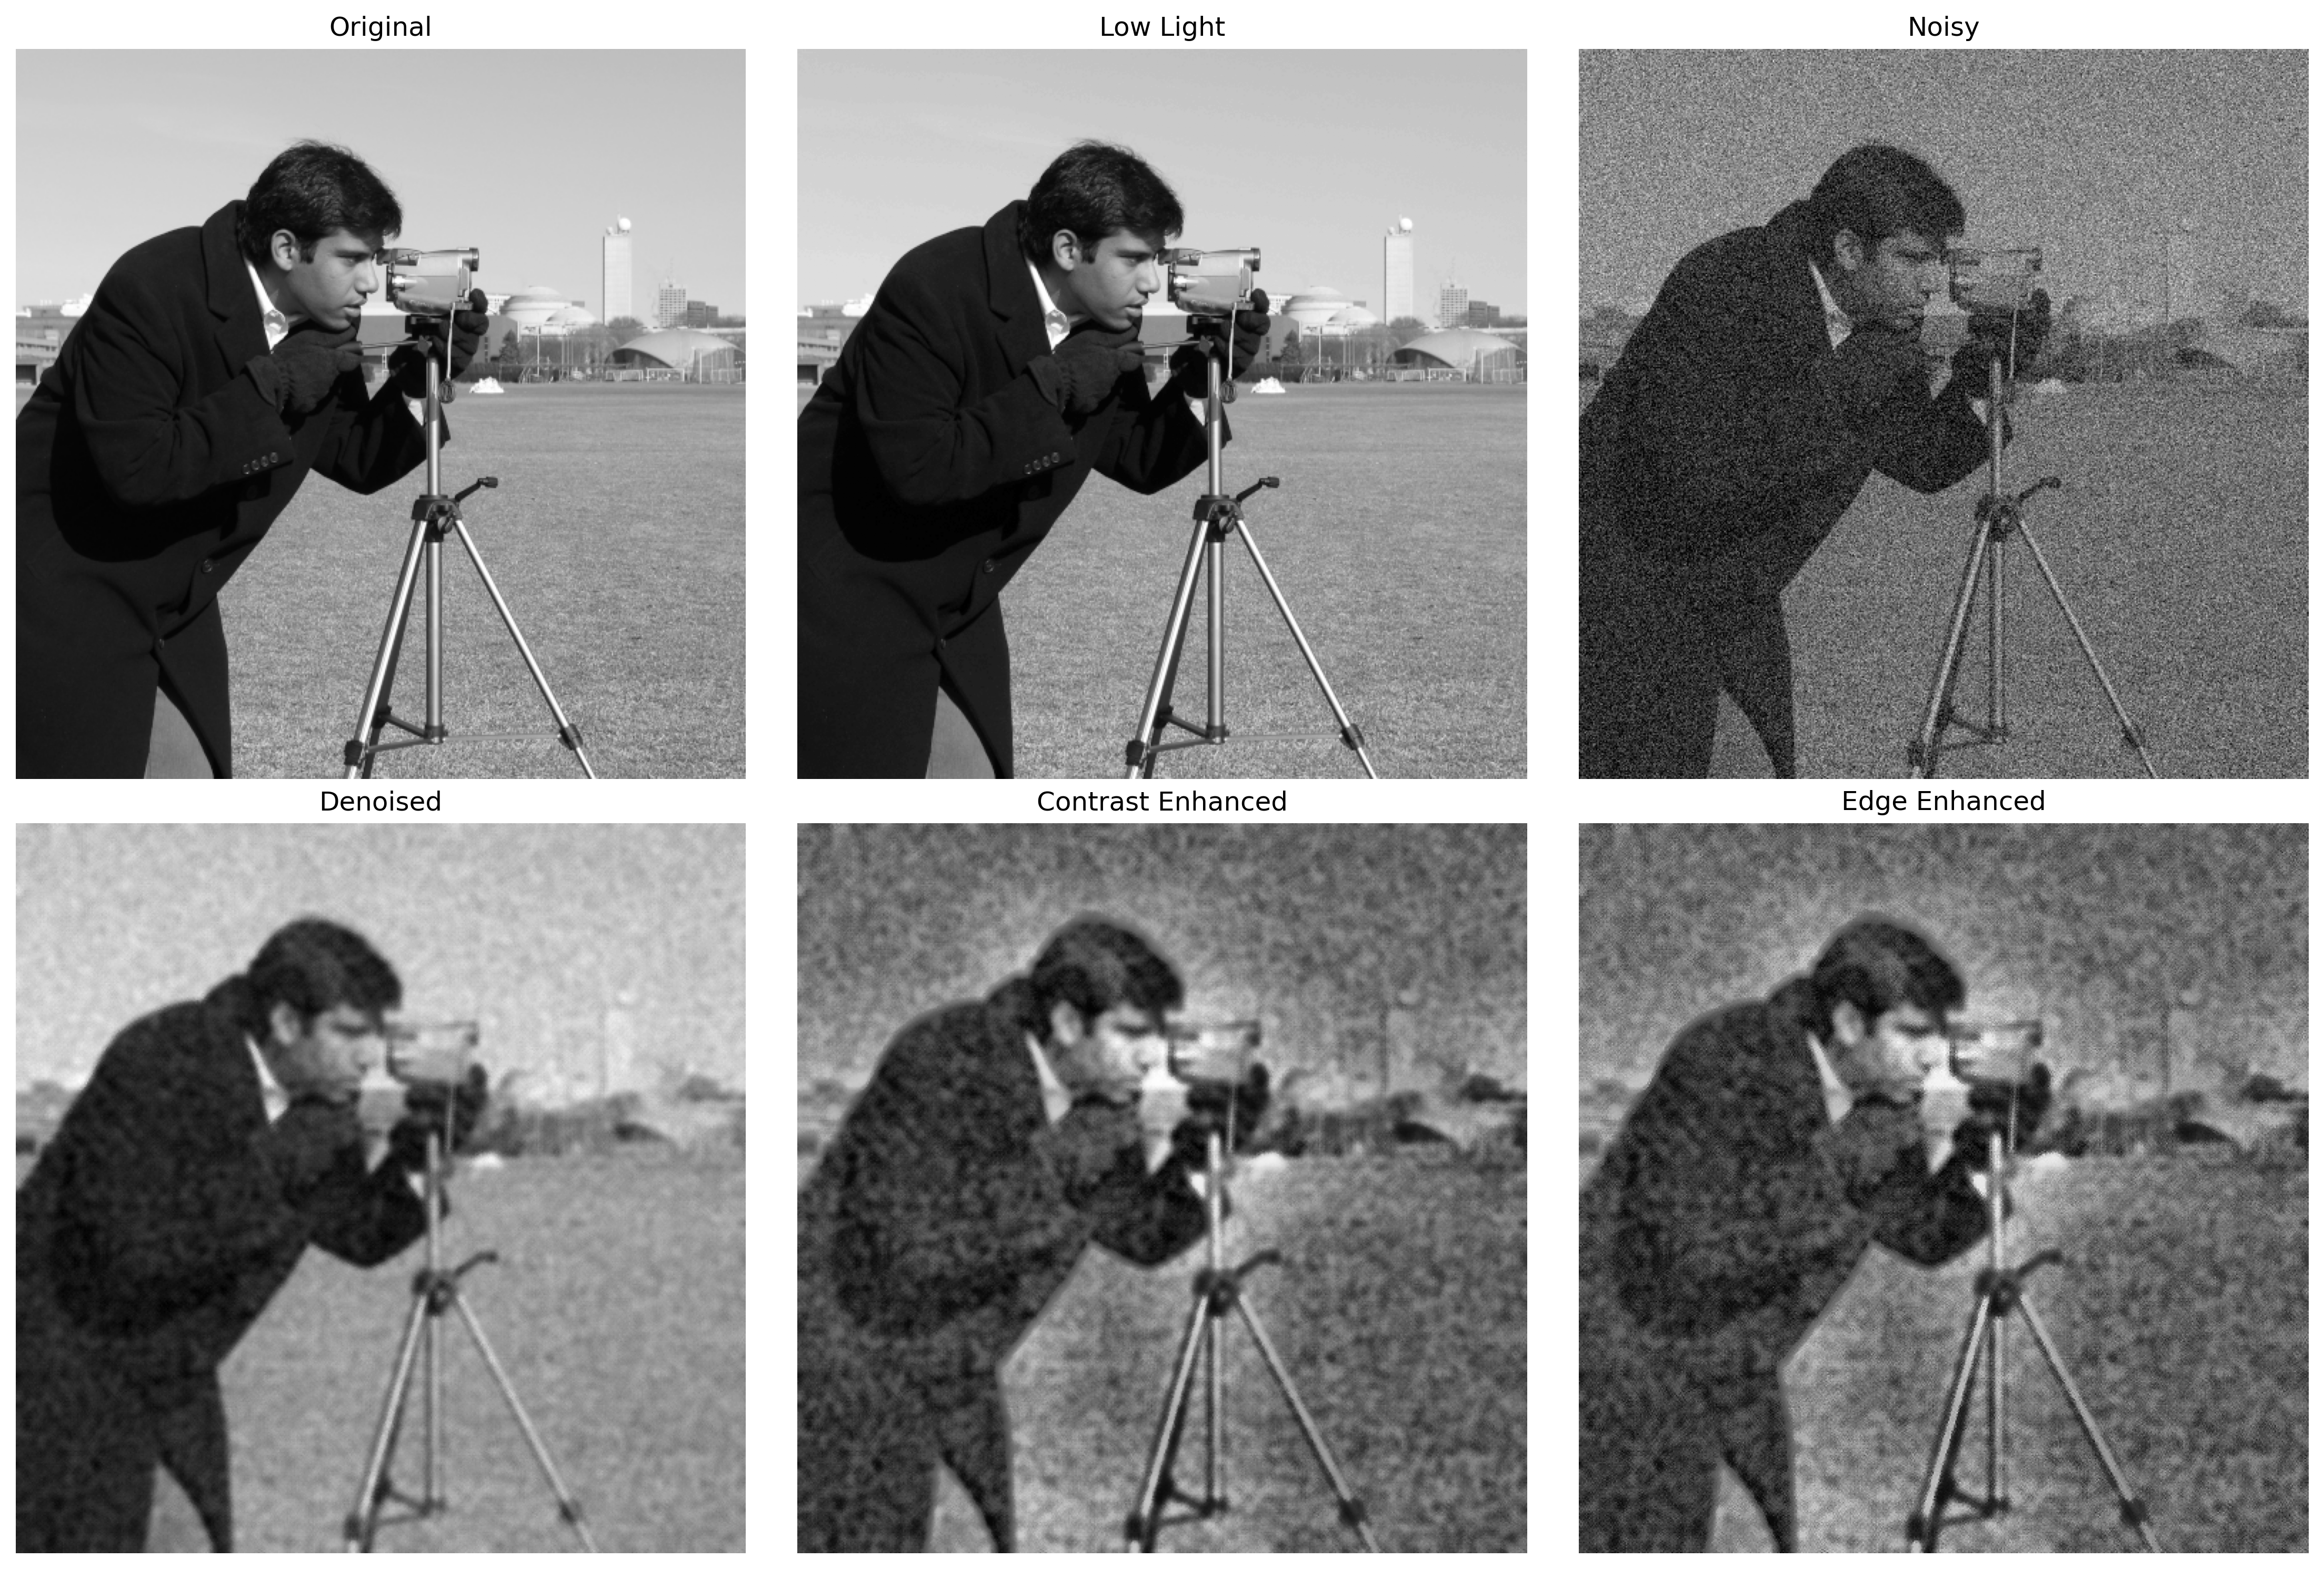
\includegraphics[width=\textwidth]{../figures/surveillance_enhancement.png}\\
\centering{\small Surveillance image enhancement: noise reduction and detail enhancement}
\end{column}
\end{columns}
\end{frame}

\section{Advanced Topics}

\begin{frame}{Adaptive and Edge-Preserving Filters}
\begin{columns}
\begin{column}{0.55\textwidth}
\textbf{Bilateral Filter:}
\begin{align}
I_{\text{filtered}}(x) &= \frac{1}{W_p} \sum_{x_i \in \Omega} I(x_i) \cdot \\
&\quad f_r(||I(x_i) - I(x)||) \cdot g_s(||x_i - x||)
\end{align}

Where:
\begin{itemize}
\item $f_r$ = range kernel (intensity similarity)
\item $g_s$ = spatial kernel (geometric closeness)
\item $W_p$ = normalization factor
\end{itemize}

\textbf{Non-local Means:}
$$\text{NL}(I)(x) = \sum_{y \in \Omega} w(x,y) I(y)$$

\textbf{Weight function:}
$$w(x,y) = \frac{1}{Z(x)} e^{-\frac{||v(N_x) - v(N_y)||^2}{h^2}}$$
\end{column}
\begin{column}{0.4\textwidth}
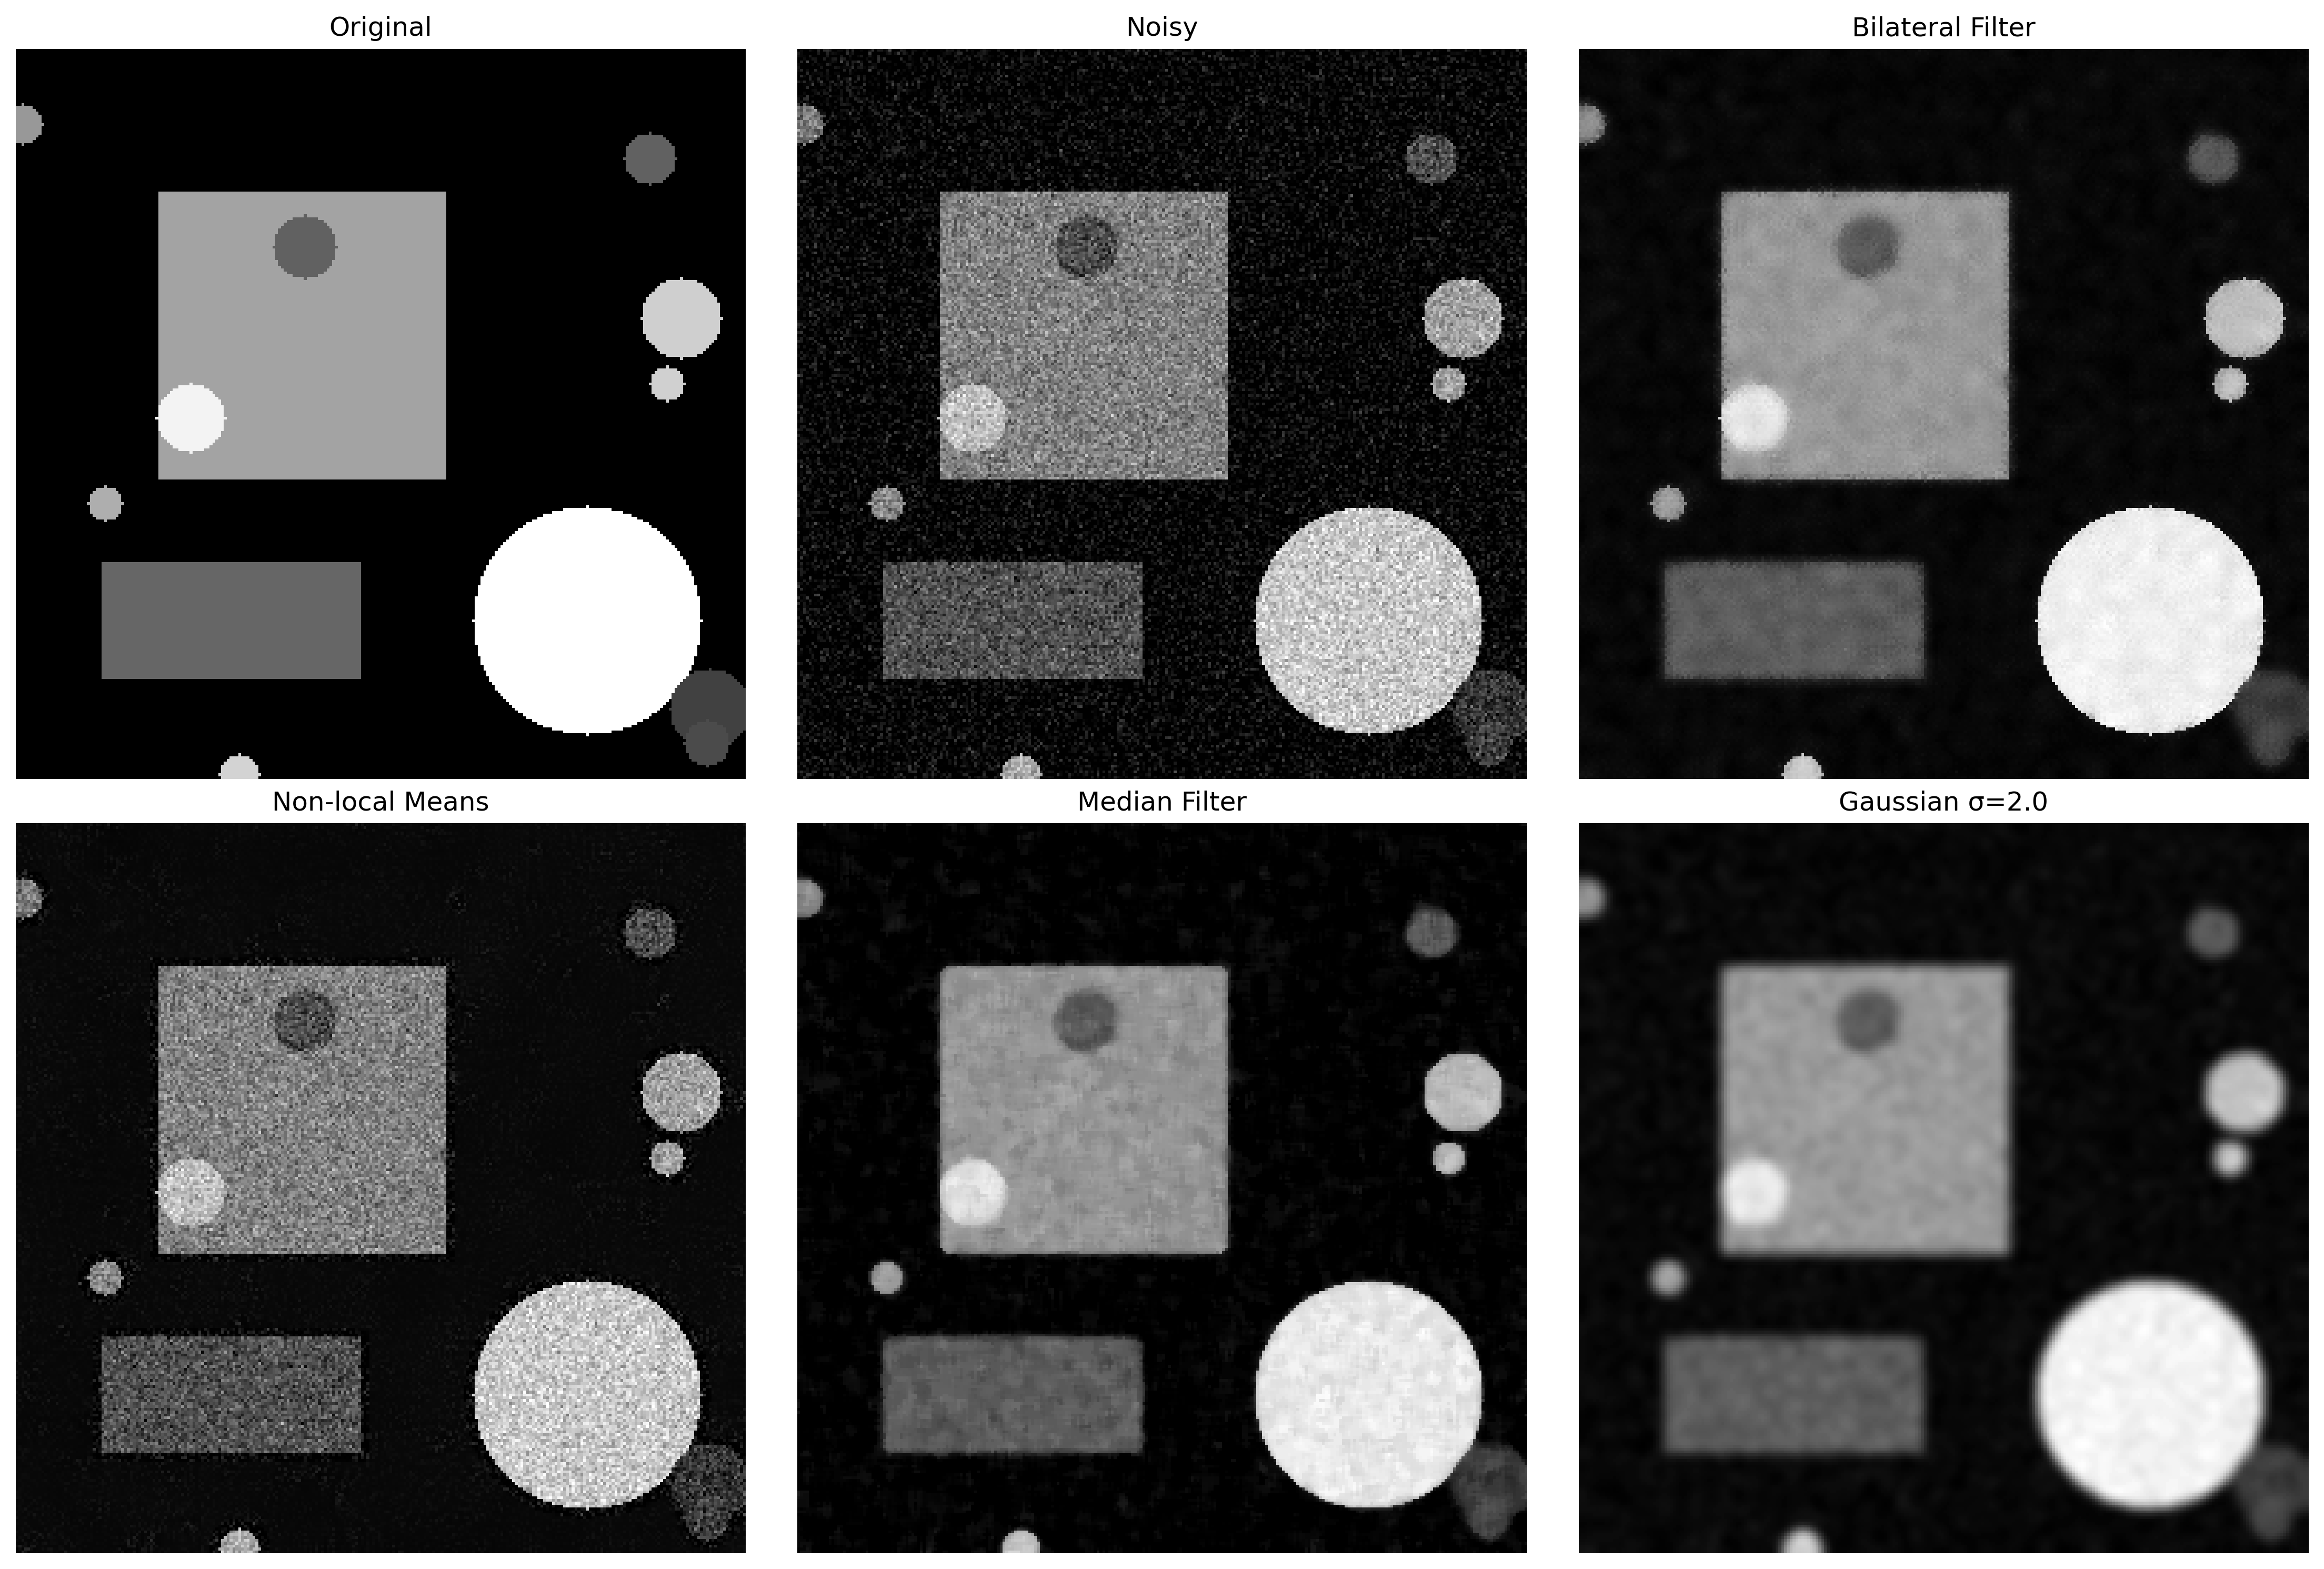
\includegraphics[width=\textwidth]{../figures/adaptive_filtering.png}\\
\centering{\small Adaptive filtering: bilateral, non-local means, and edge-preserving techniques}
\end{column}
\end{columns}
\end{frame}

\begin{frame}{Unsharp Masking and Sharpening}
\begin{columns}
\begin{column}{0.55\textwidth}
\textbf{Unsharp Masking Process:}
\begin{enumerate}
\item Create blurred version: $f_{\text{blur}} = f \star G_\sigma$
\item Generate mask: $\text{mask} = f - f_{\text{blur}}$
\item Add scaled mask: $f_{\text{sharp}} = f + k \cdot \text{mask}$
\end{enumerate}

\textbf{Mathematical Form:}
$$g(x,y) = f(x,y) + k[f(x,y) - \bar{f}(x,y)]$$

Where:
\begin{itemize}
\item $k$ = sharpening strength
\item $\bar{f}(x,y)$ = blurred image
\end{itemize}

\textbf{Laplacian Sharpening:}
$$g(x,y) = f(x,y) - \nabla^2 f(x,y)$$
\end{column}
\begin{column}{0.4\textwidth}
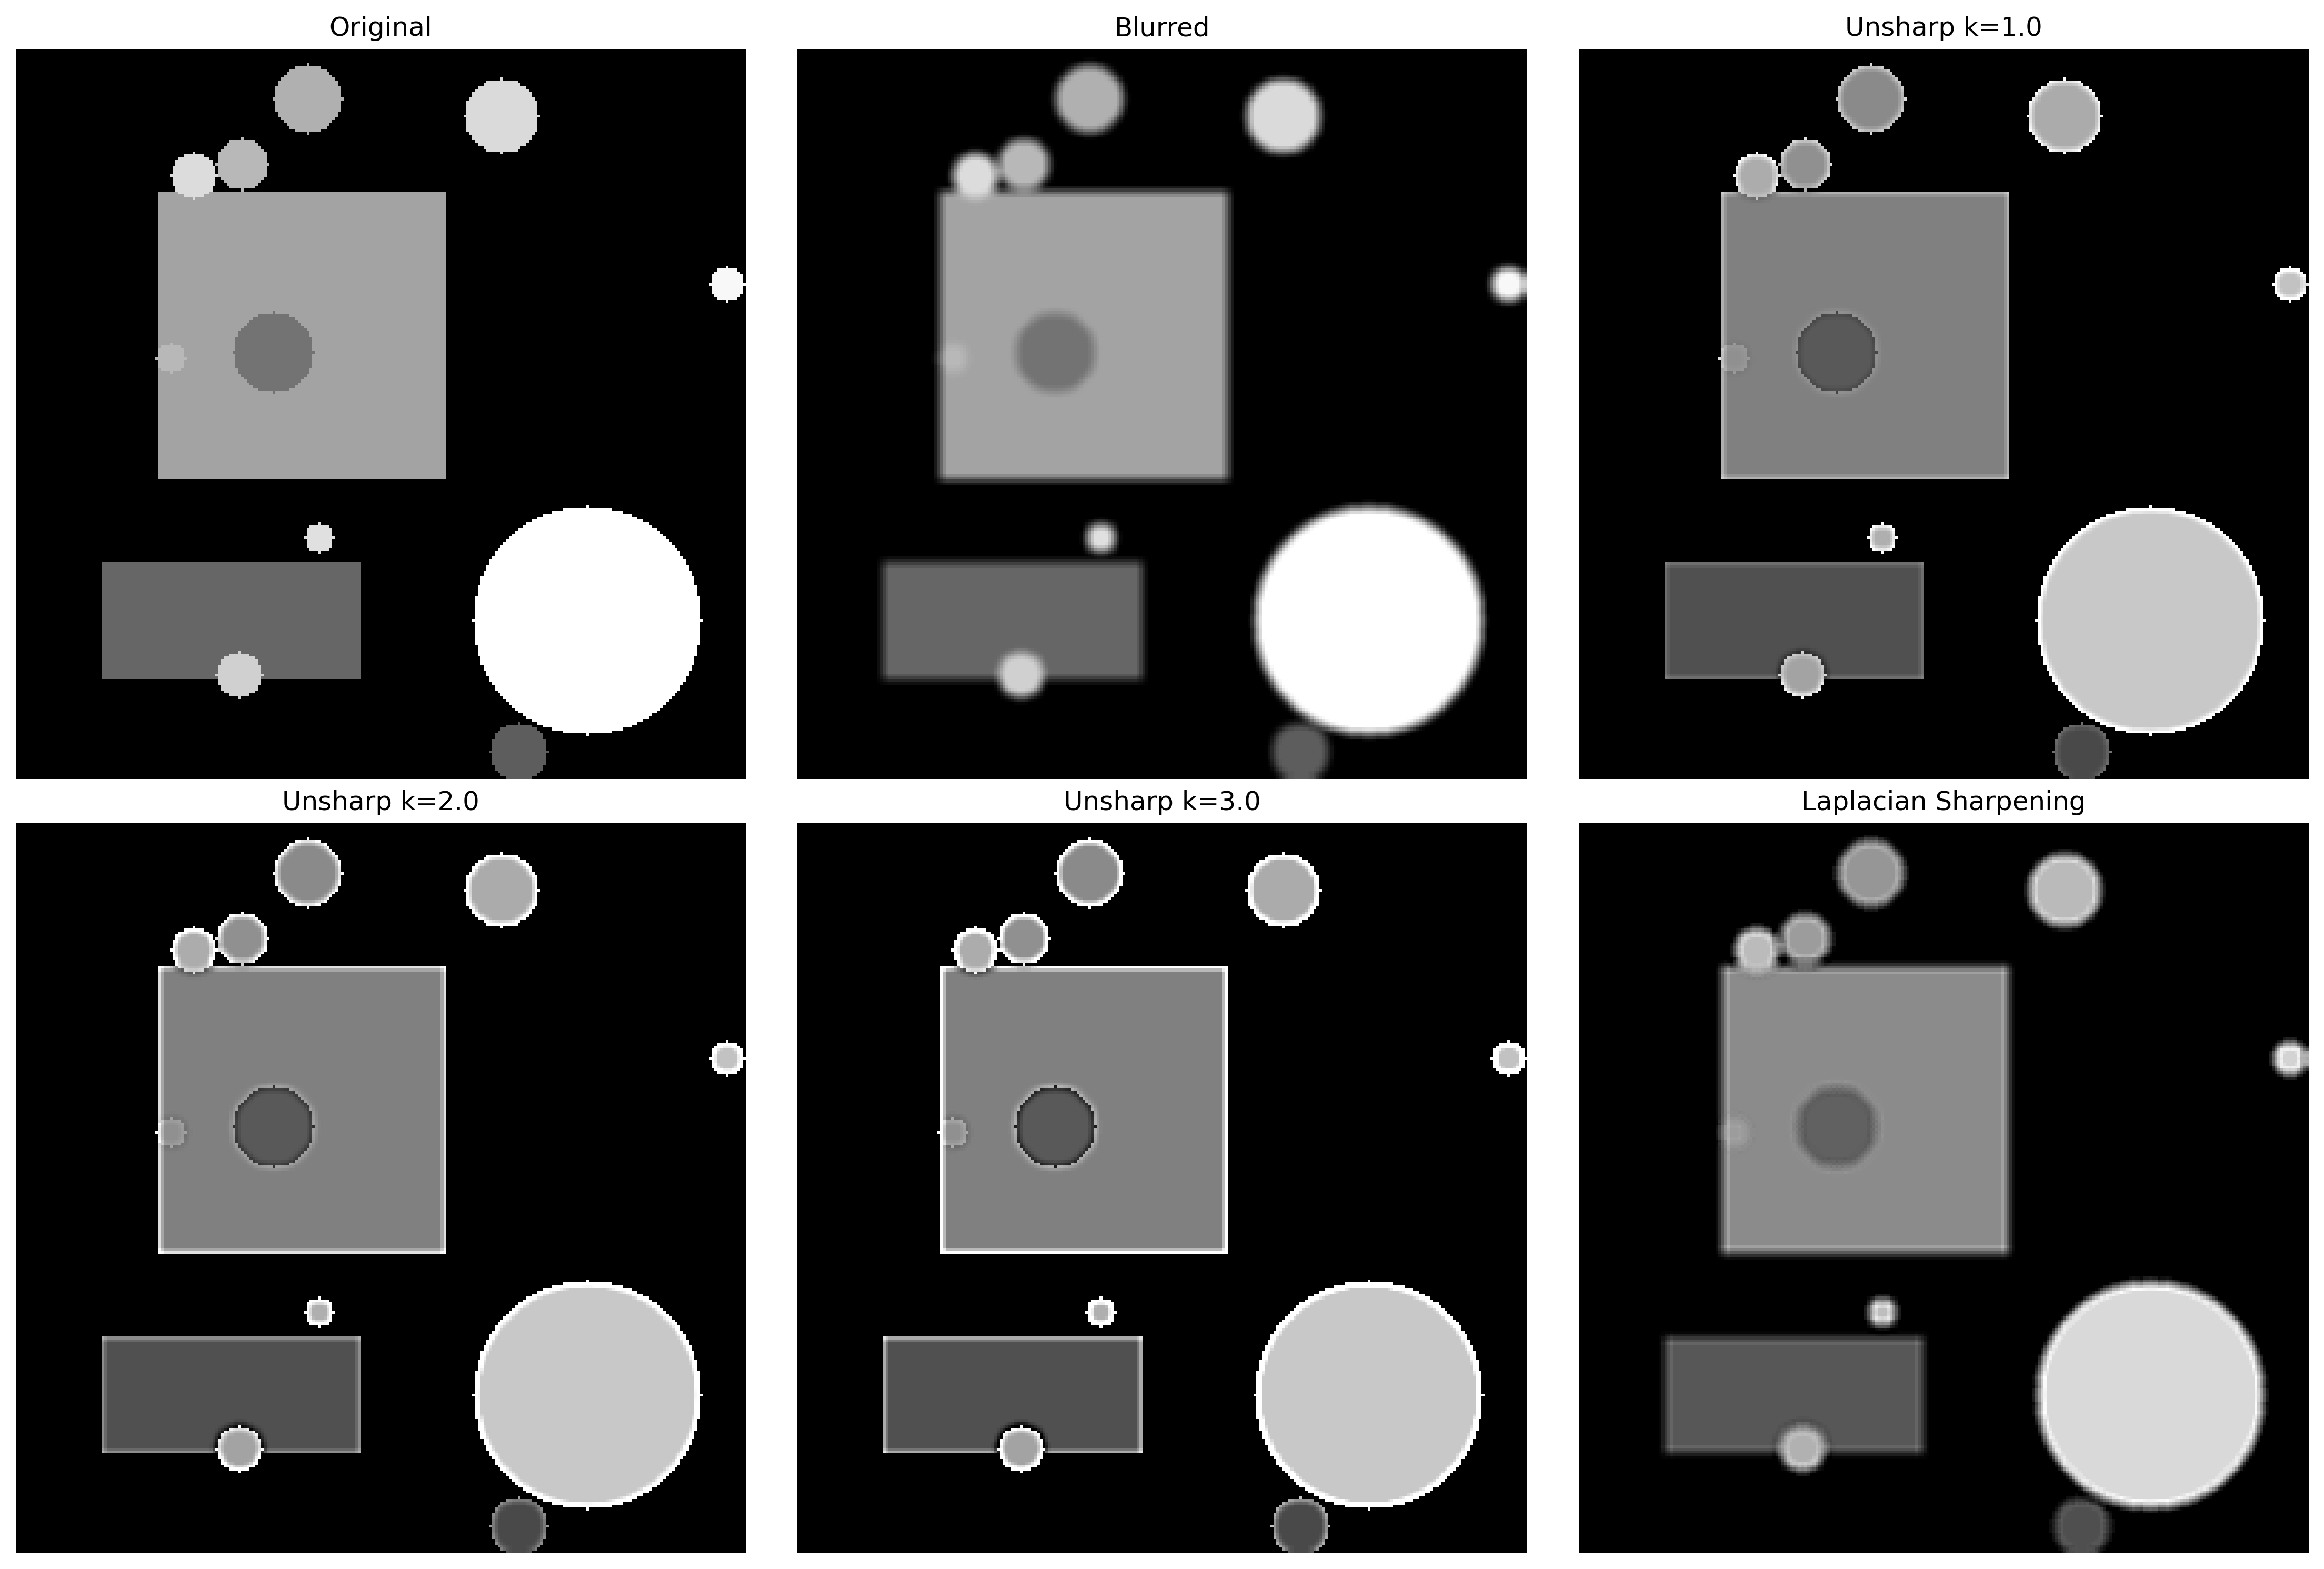
\includegraphics[width=\textwidth]{../figures/unsharp_masking.png}\\
\centering{\small Unsharp masking process: original, blurred, mask, and sharpened result}
\end{column}
\end{columns}
\end{frame}

\begin{frame}{Morphological Operations}
\begin{columns}
\begin{column}{0.55\textwidth}
\textbf{Basic Operations:}
\begin{align}
\text{Erosion:} \quad A \ominus B &= \{z | (B)_z \subseteq A\} \\
\text{Dilation:} \quad A \oplus B &= \{z | (\hat{B})_z \cap A \neq \emptyset\}
\end{align}

\textbf{Compound Operations:}
\begin{align}
\text{Opening:} \quad A \circ B &= (A \ominus B) \oplus B \\
\text{Closing:} \quad A \bullet B &= (A \oplus B) \ominus B
\end{align}

\textbf{Applications:}
\begin{itemize}
\item Noise removal
\item Shape analysis
\item Object separation
\item Texture analysis
\end{itemize}
\end{column}
\begin{column}{0.4\textwidth}
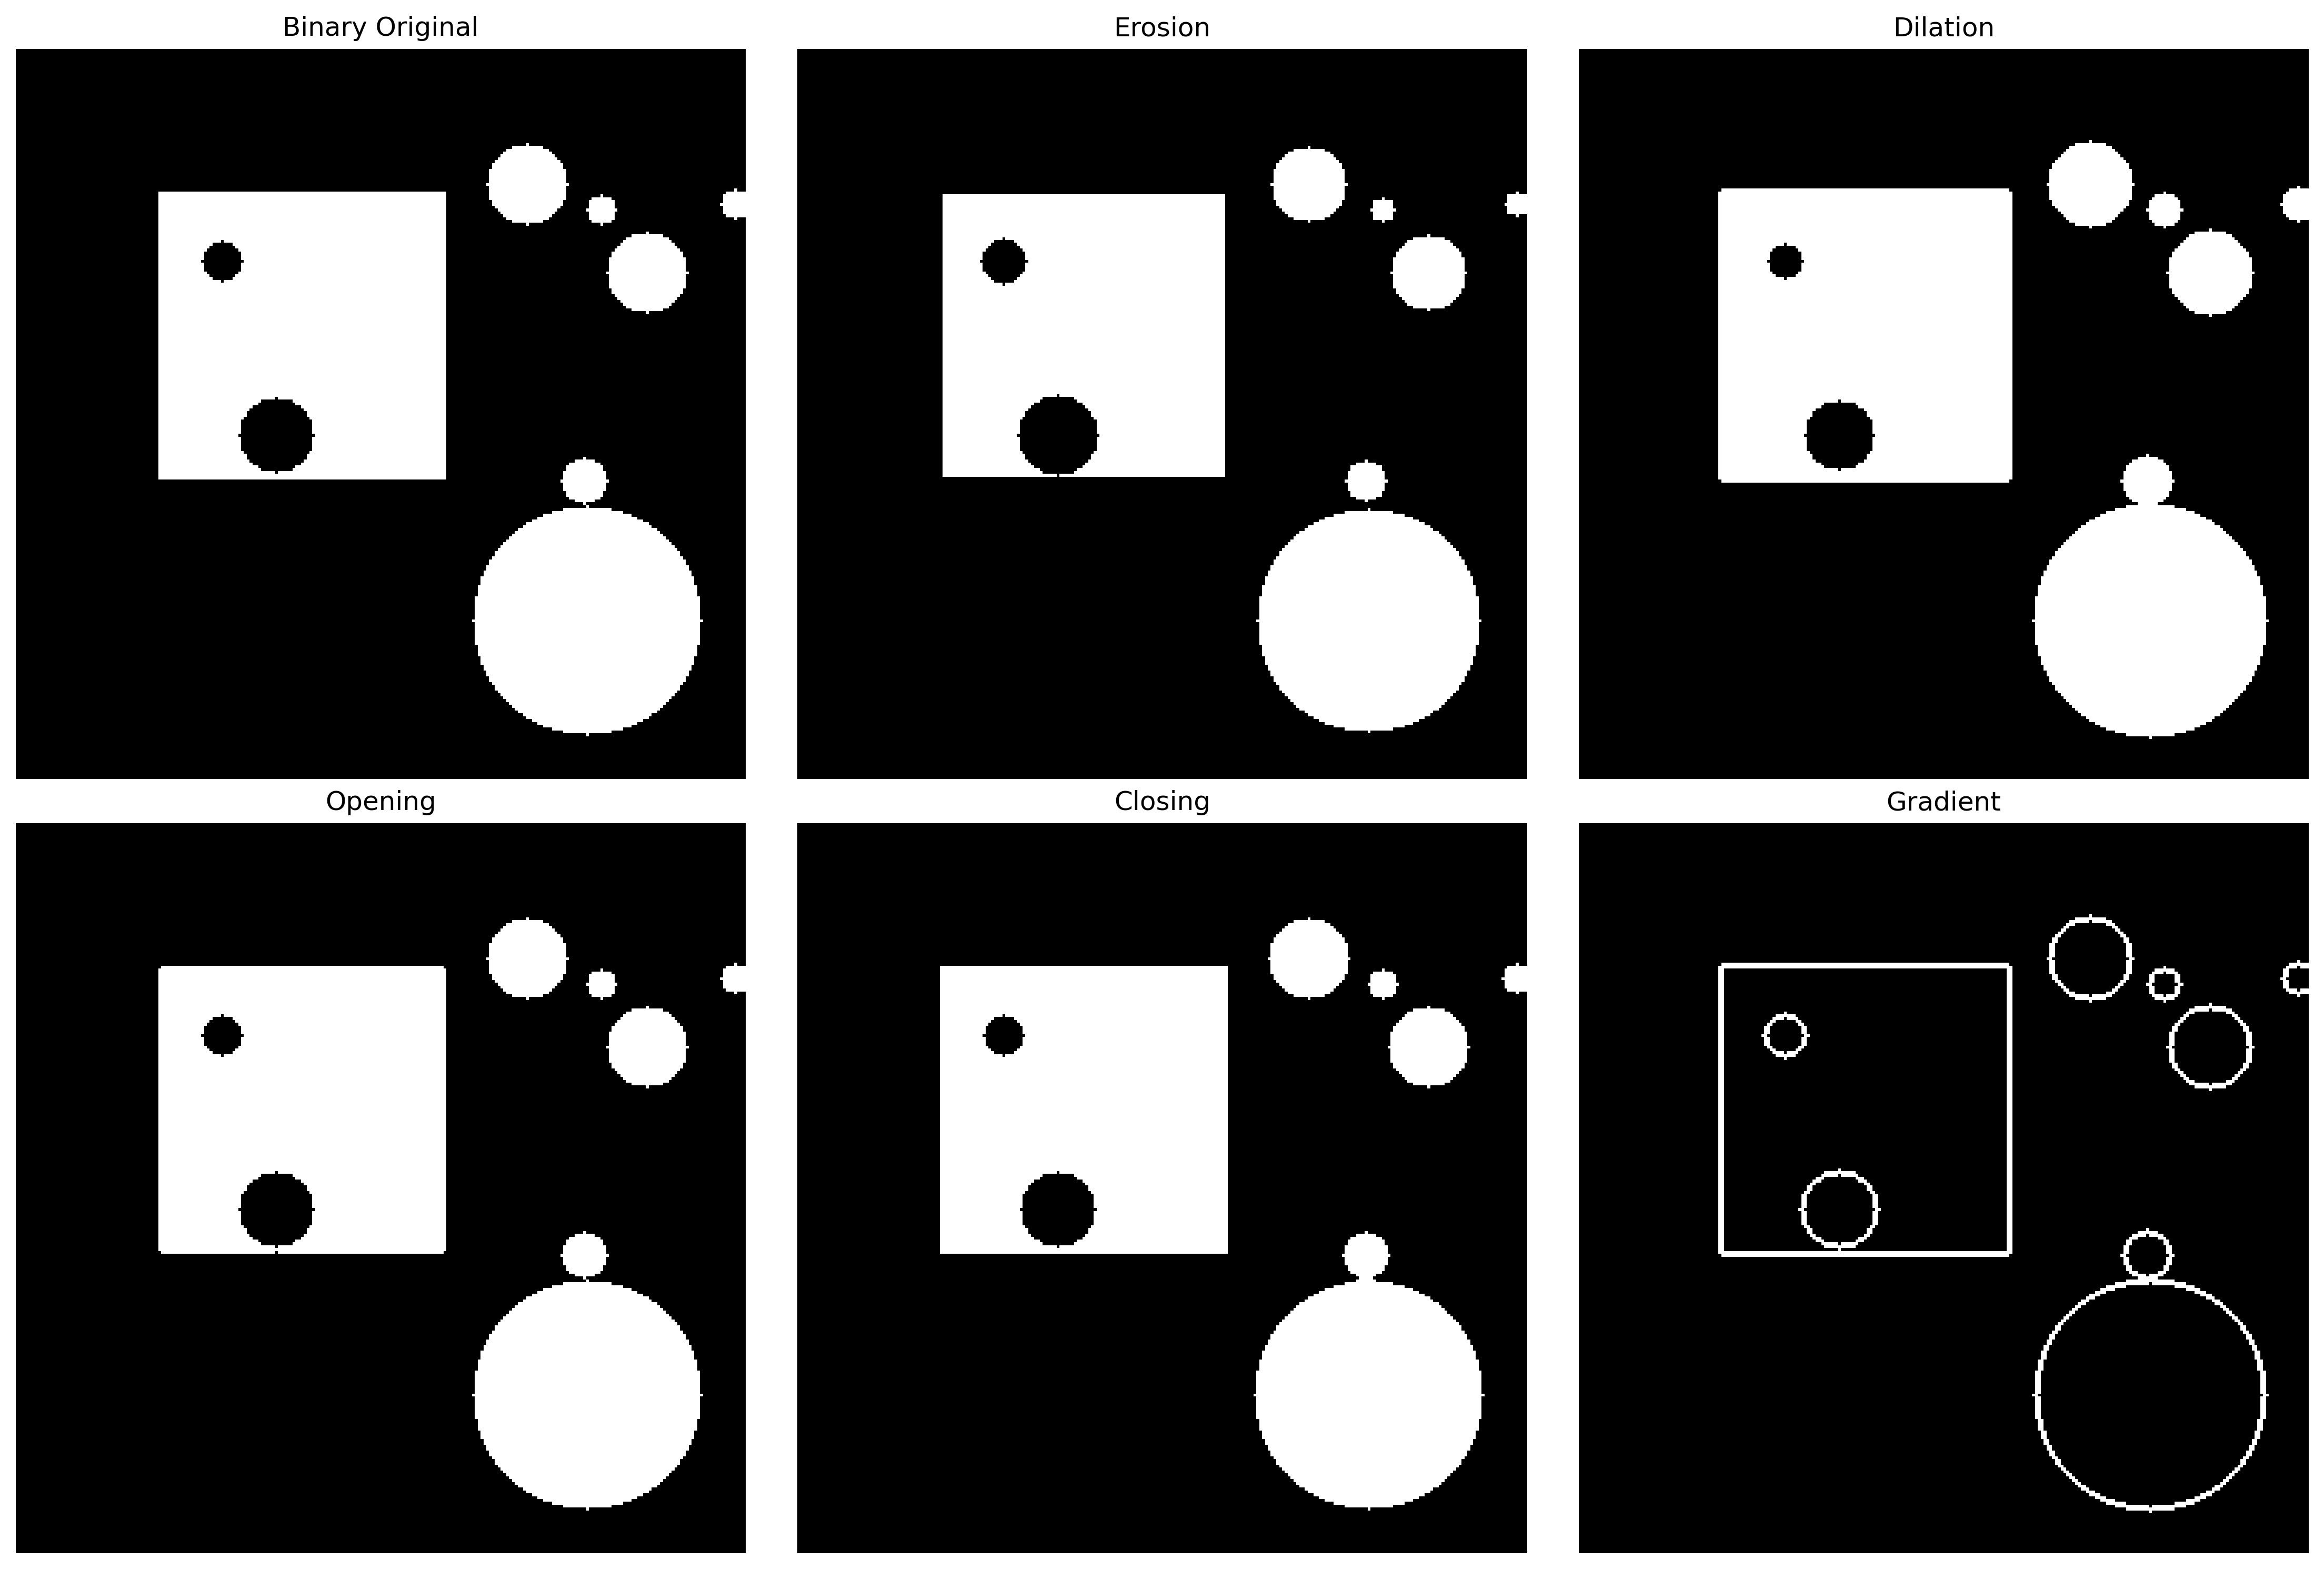
\includegraphics[width=\textwidth]{../figures/morphological_operations.png}\\
\centering{\small Morphological operations: erosion, dilation, opening, and closing effects}
\end{column}
\end{columns}
\end{frame}

\section{Best Practices}

\begin{frame}{Common Pitfalls and Solutions}
\begin{alertblock}{Pitfall 1: Over-enhancement}
\textbf{Problem:} Excessive enhancement creates artifacts
\textbf{Solution:} Use moderate parameters, validate results
\end{alertblock}

\begin{alertblock}{Pitfall 2: Noise amplification}
\textbf{Problem:} Enhancement amplifies noise
\textbf{Solution:} Apply noise reduction before enhancement
\end{alertblock}

\begin{alertblock}{Pitfall 3: Loss of detail}
\textbf{Problem:} Aggressive smoothing removes important details
\textbf{Solution:} Use edge-preserving filters (bilateral, NLM)
\end{alertblock}

\begin{alertblock}{Pitfall 4: Inconsistent processing}
\textbf{Problem:} Different enhancement for similar images
\textbf{Solution:} Develop standardized pipelines, use adaptive methods
\end{alertblock}
\end{frame}

\begin{frame}{Quality Assessment Metrics}
\begin{columns}
\begin{column}{0.5\textwidth}
\textbf{Objective Metrics:}
\begin{align}
\text{PSNR} &= 20 \log_{10} \frac{255}{\sqrt{\text{MSE}}} \\
\text{SNR} &= 10 \log_{10} \frac{\sigma_{\text{signal}}^2}{\sigma_{\text{noise}}^2} \\
\text{Contrast} &= \sigma_{\text{intensity}}
\end{align}

\textbf{Perceptual Metrics:}
\begin{itemize}
\item Edge preservation
\item Detail enhancement
\item Artifact reduction
\item Visual naturalness
\end{itemize}
\end{column}
\begin{column}{0.45\textwidth}
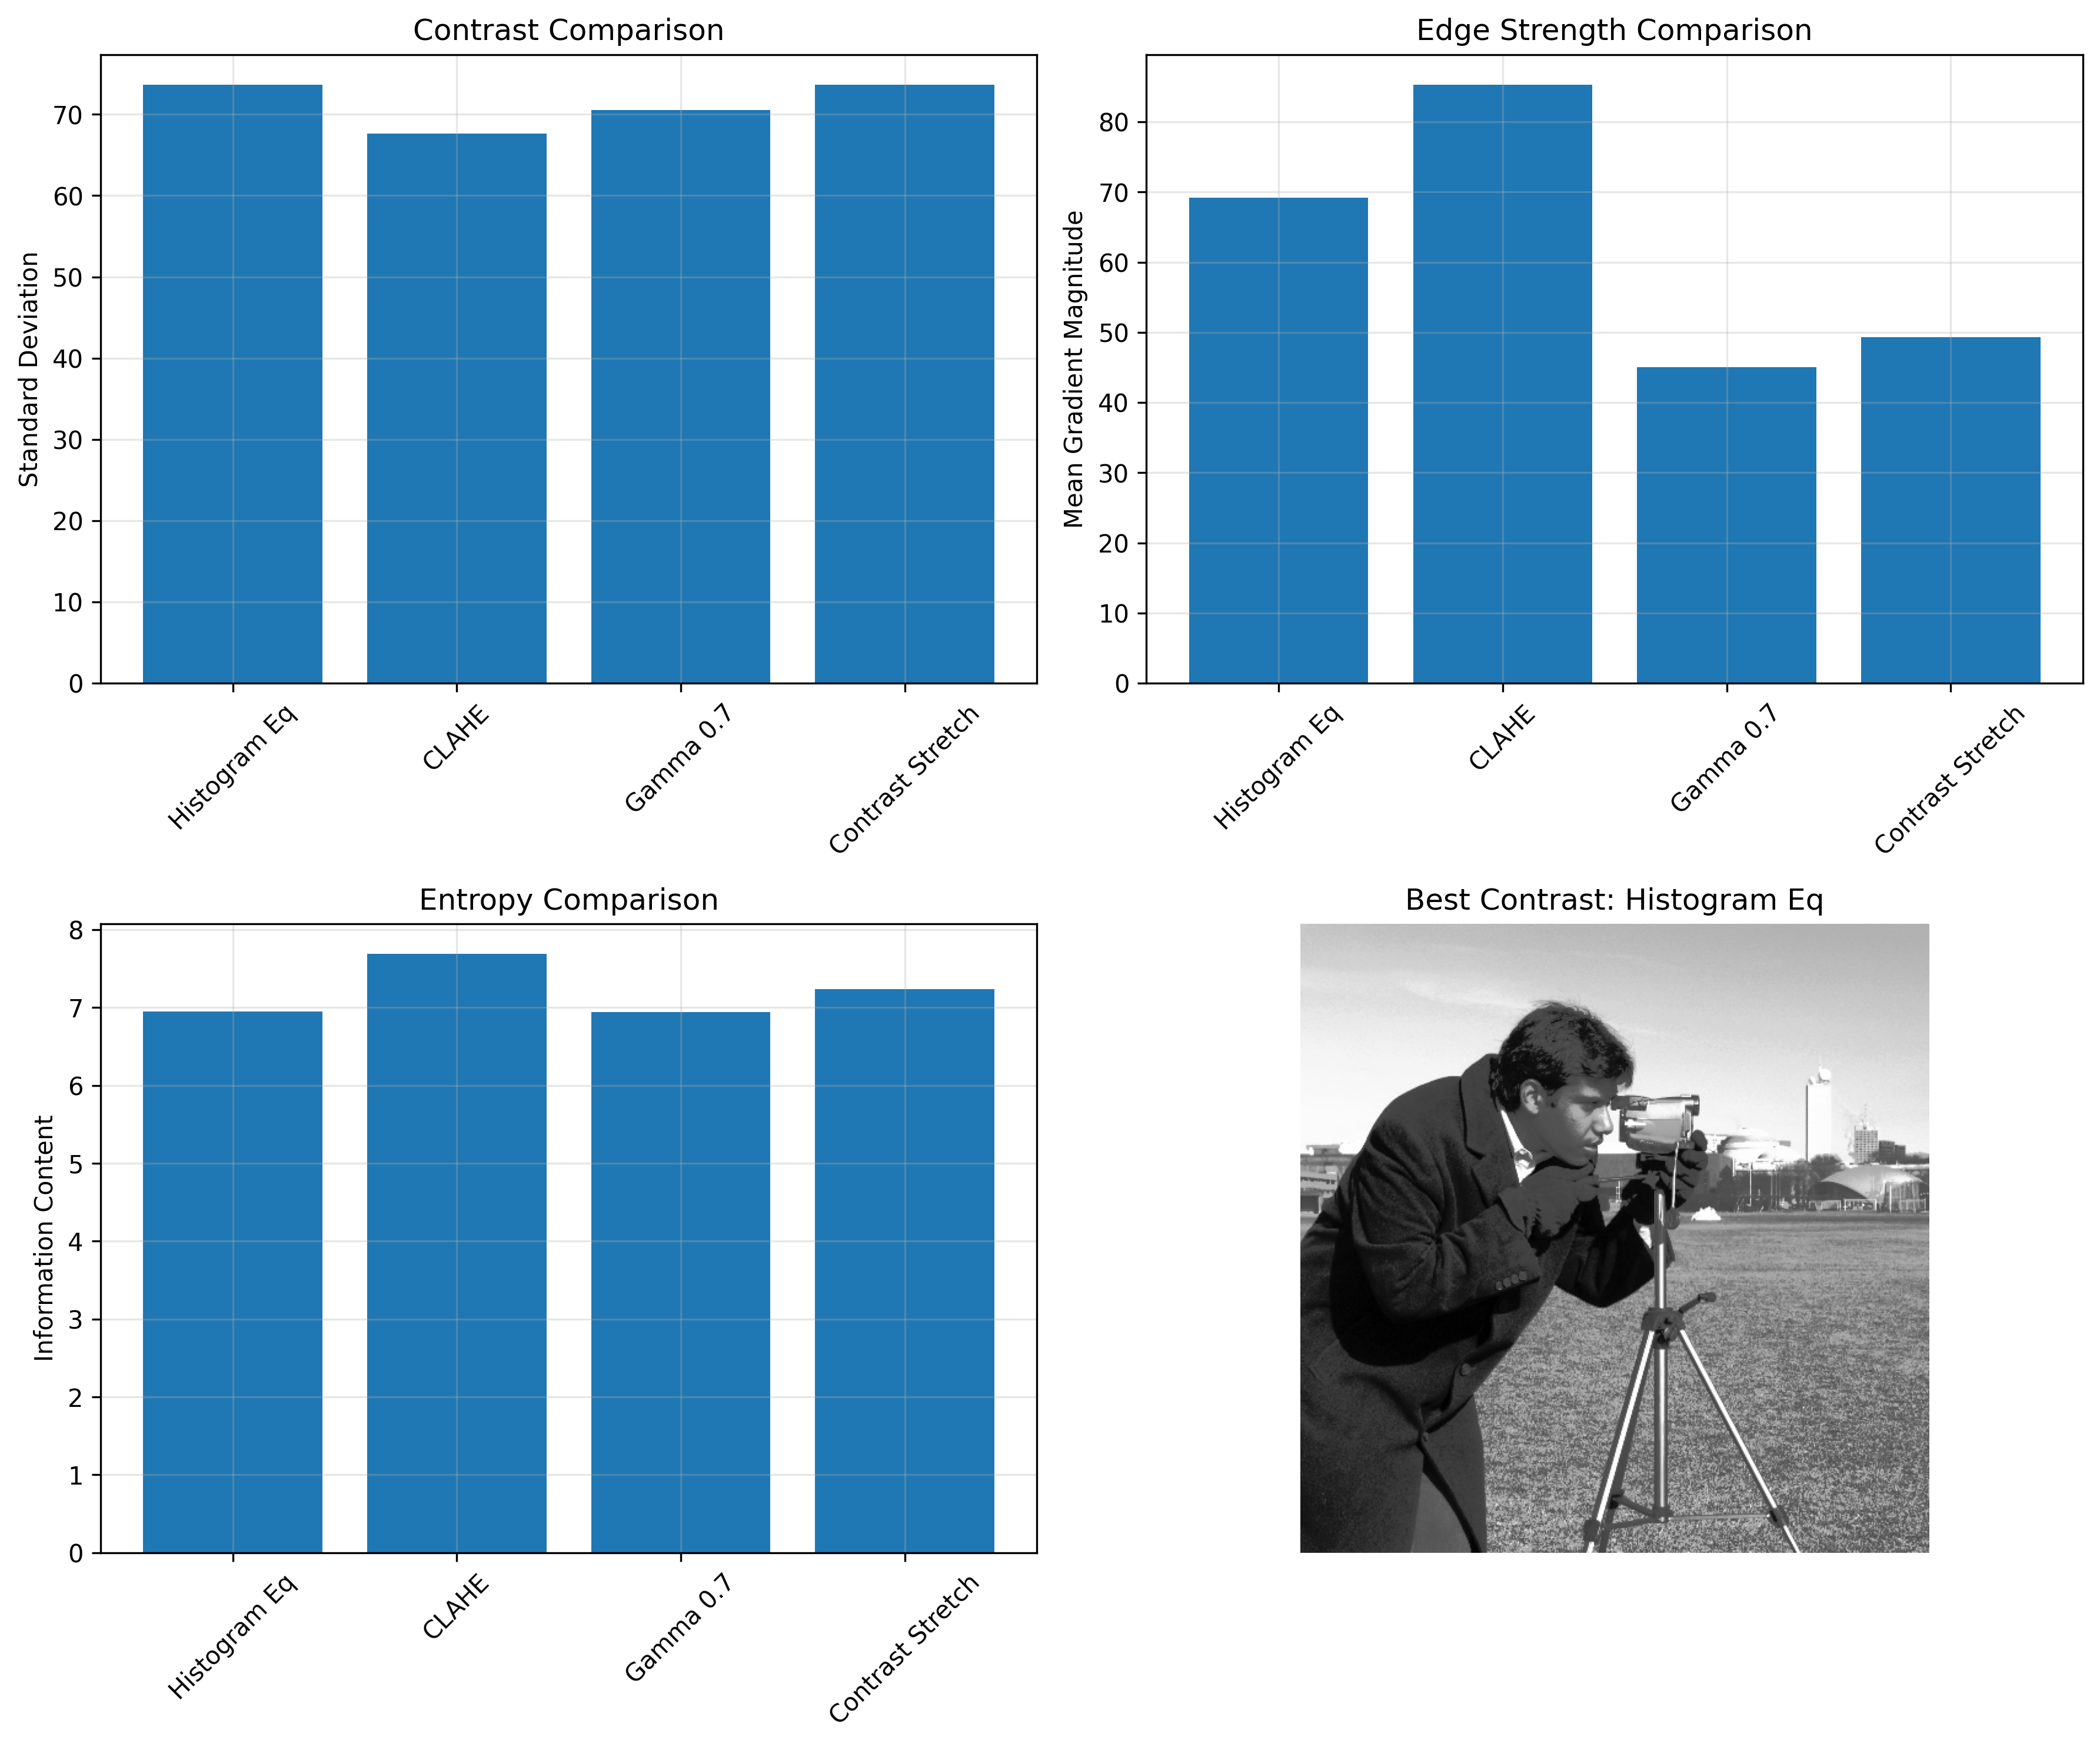
\includegraphics[width=\textwidth]{../figures/quality_metrics.png}\\
\centering{\small Quality assessment metrics: PSNR, SSIM, and visual comparison results}
\end{column}
\end{columns}
\end{frame}

\begin{frame}{Processing Guidelines}
\textbf{General Pipeline:}
\begin{enumerate}
\item \textbf{Assessment:} Analyze image characteristics
\item \textbf{Preprocessing:} Noise reduction if needed
\item \textbf{Enhancement:} Apply appropriate techniques
\item \textbf{Validation:} Check results quantitatively
\item \textbf{Refinement:} Adjust parameters as needed
\end{enumerate}

\textbf{Parameter Selection:}
\begin{itemize}
\item Start with conservative values
\item Validate on representative images
\item Consider computational constraints
\item Maintain consistency across datasets
\end{itemize}

\textbf{Real-time Considerations:}
\begin{itemize}
\item Optimize algorithms for speed
\item Use lookup tables when possible
\item Consider hardware acceleration
\item Balance quality vs. speed
\end{itemize}
\end{frame}

\section{Summary}

\begin{frame}{Key Takeaways}
\begin{columns}
\begin{column}{0.48\textwidth}
\textbf{Fundamental Concepts:}
\begin{itemize}
\item Enhancement improves image quality
\item Point operations modify pixels
\item Spatial operations use neighborhoods
\item Frequency domain transforms
\end{itemize}

\textbf{Essential Techniques:}
\begin{itemize}
\item \textbf{Histogram equalization}
\item \textbf{Gamma correction}
\item \textbf{Spatial filtering}
\item \textbf{Edge detection}
\end{itemize}
\end{column}
\begin{column}{0.48\textwidth}
\textbf{Best Practices:}
\begin{itemize}
\item Choose based on image characteristics
\item Validate using metrics
\item Avoid over-enhancement
\item Consider computational cost
\end{itemize}
\end{column}
\end{columns}
\end{frame}

\begin{frame}{Next Steps}
\textbf{Advanced Topics to Explore:}
\begin{itemize}
\item Frequency domain enhancement
\item Multi-scale processing
\item Machine learning-based enhancement
\item Real-time implementation
\end{itemize}

\textbf{Integration with Other Topics:}
\begin{itemize}
\item Image restoration and denoising
\item Feature detection and matching
\item Image segmentation
\item Computer vision applications
\end{itemize}

\textbf{Practical Applications:}
\begin{itemize}
\item Medical image analysis
\item Remote sensing
\item Digital photography
\item Video processing
\end{itemize}
\end{frame}

\begin{frame}[standout]
\Large
\textbf{Questions \& Discussion}

\vspace{1cm}
\normalsize
Ready for hands-on practice?\\
Check out the interactive notebook!
\end{frame}

\end{document}